\documentclass[12pt,a4paper]{report}

%Set language
\usepackage[english]{babel}
\usepackage{enumerate}

% To import and adjust images
\usepackage{graphicx}
\usepackage[export]{adjustbox}
\usepackage[center]{caption}
\usepackage{subcaption}
\usepackage{float}
\usepackage{tabularx}

% To use monospaced font
\usepackage{courier}

% To build a clickable Toc
\usepackage{color} %May be necessary if you want to color links
\usepackage{hyperref}
\hypersetup{
    colorlinks=true, %set true if you want colored links
    linktoc=all,     %set to all if you want both sections and subsections linked
    linkcolor=black,  %choose some color if you want links to stand out
    urlcolor = black
}

%To load PoLitecnico's logo
\usepackage{titling}

% Command to hide subsections in the Toc
\setcounter{tocdepth}{1}

% I don't like dots in the Toc
\usepackage{tocloft}
\renewcommand{\cftdot}{}

%To improve the tables
\usepackage[table]{xcolor}

% Path relative to the .tex file containing the \includegraphics command
\graphicspath{ {./images/} }

% To change the ToC title
\addto\captionsenglish{ \renewcommand {\contentsname} {Table of
contents}}

%logo
\pretitle{
	 \begin{center}
	 \LARGE
	 
\includegraphics[width = 0.6\textwidth]{logo}\\[\bigskipamount]
}
\posttitle{\end{center}}

% Here we go
\title{SafeStreets - DD \\ \large version 1.0}
\author{Frangi Alberto, Fucci Tiziano}
\date{A.Y. 2019/2020}
\begin{document}
	\maketitle
	%Index
	\tableofcontents
	\chapter{Introduction}
		\section{Purpose}
			The purpose of this document consists of giving more technical details than the RASD concerning the SafeStreets
			system.\\
			The RASD document completely describes the system in terms of functional and nonfunctional requirements and
			serves as a contractual basis between the customer and the developer and it must be written in the language of
			the customer's domain of business/expertise, the DD's purpose instead is to provide a description for how the new
			system will be constructed, it provides a description of the system architecture, software, hardware, database
			design, and security.\\
			In particular this document will explain the following topics:
			\begin{itemize}
				\item High level architecture and its components' requirements;
				\item Run-time behavior;
				\item Design patterns;
				\item Additional user interfaces information;
				\item Implementation, integration and testing plan.
			\end{itemize}
		\section{Scope}
			Safestreet is an application to be used both from civilians (users) and authorities, in order to help the latter and
			reduce traffic violations. Registered authorities can automatically receive reports made by users, so the service acts
			as an intermediary. The next paragraph gives a more formal description of system's architecture.

		\section{Definitions, Acronyms, Abbreviations}
			\subsection{Definitions}
				\begin{itemize}
				\item \textbf{User}: a civilian customer that can use the application to:
					\begin{itemize}
					\item notify authorities of some violation;
					\item check which are the most dangerous (i.e. with the most violations) streets.
					\end{itemize}
				In this document, ``user", ``citizen" and ``civiian" are completely equivalent, where not specified.
				\item \textbf{Authority}: a member of the local police who has access to reports made by users. The
					authorities evaluate the reports sent by the user to determine if the violation stands.
				\item \textbf{Report}: a message consisting of:
					\begin{itemize}
					\item a picture showing the car in order to show the occurring violation;
					\item date and time of the picture;
					\item GPS position of the place where the violation occurred;
					\item the street where the violation occurred (automatically retrieved from the geographical position);
					\item the type of the violation (input by the user)
					\end{itemize}
				\item \textbf{Available}: a report is available for an authority if its position is within the municipality assigned
					to the authority.
				\item \textbf{Violation}: a situation that, according to the user who sent the report, is a violation of the
					traffic laws.
				\item \textbf{Intervention}: a brief text suggesting a possible solution in order to improve safety and
					discourage future violations.
				\end{itemize}
			\subsection{Acronyms}
				\begin{itemize}
				\item \textbf{API}: \emph{Application Programming Interface.}
				\item \textbf{GPS}: \emph{Global Positioning System.}
				\item \textbf{UI}: \emph{User Interface.}
				\item \textbf{RASD:} \emph{Requirements Analysis and Specifications Document}
				\item \textbf{DD:} \emph{Design Document}
				\item \textbf{DMZ:} \emph{DeMilitarized Zone}
				\item \textbf{PKC}: \emph{Public Key Cryptography.}
				\item \textbf{AES}: \emph{Advanced Encryption Standard.}
				\item \textbf{XML}: \emph{eXtensible Markup Language.}
				\item \textbf{HTML}: \emph{HyperText Markup Language.}
				\item \textbf{OCR}: \emph{Optical Character Recognition.}
				\item \textbf{DB}: \emph{Data Base.}				
				\item \textbf{SS}: \emph{SafeStreets.}	
				\item \textbf{DBMS}: \emph{Data Base Management System.}
				\item \textbf{RDBMS}: \emph{Relational Data Base Management System.}
				\item \textbf{UML}: \emph{Unified Modeling Language.}
				\item \textbf{REST}: \emph{REpresentational State Transfer.}
				\item \textbf{SHA-3}: \emph{Secure Hash Algorithm 3.}
				\end{itemize}
		\section{Revision History}
			\begin{itemize}
				\item \textbf{Version 1.0:}
				\begin{itemize}
					\item First release.
				\end{itemize}
			\end {itemize}
		\section{Reference Documents}
			\begin{itemize}
				\item \textbf{Specification document:} "Mandatory project assignment AY 2019/20".
			\end{itemize}
		\section{Document Structure}
			\begin{itemize}
				\item \textbf{Chapter 1} provides a brief explanation on the DD purpose and a quick introduction
					SafeStreets.
				\item \textbf{Chapter 2} aims to provide a description of the system's architecture.
				\item \textbf{Chapter 3} specifies the design of user interfaces and describes the user-application
					interaction.
				\item \textbf{Chapter 4} contains requirements traceability.
				\item \textbf{Chapter 5} describes the implementation plan.
				\item \textbf{Chapter 6} shows the effort of each group member.
				\item \textbf{Chapter 7} contains all the references used to make this document.
			\end{itemize}
	%end of first chapter

	\chapter{Architectural design}
		\section{Overview:	high-level	components	and	their	interaction}
	The application is built following the principles of the three-tier architecture: the three logic layers of presentation, 				application and data access rely on three corresponding hardware layers. This architecture is prefered to one-tier and 			two-tier architectures due to some important characteristics, some of which are:
	\begin{itemize}
	\item \emph{Flexibility:} each tier can be manged or scaled independently at any time, without affecting the others;
	\item \emph{Scalability:} following a scale-out approach, performances can be improved through node replication, without affecting the other tiers.
	Load balancing systems distribute the working load among the nodes;
	\item \emph{Mantainability:} because each tier is independent from the others, updates or changes can be released
	without affecting the whole system;
	\item \emph{Availbility:} with this architecture, it is less likely to have failures that compromise the whole application.
	Load balancing and node replication minimize the performance loss when a failure occures.
	\end{itemize}
	These aspects will be even better explained in section 2.6.
	A general view of the system architecture is provided in the following diagram, which provides an overview of the system architecture:
	\begin{figure}[H]
			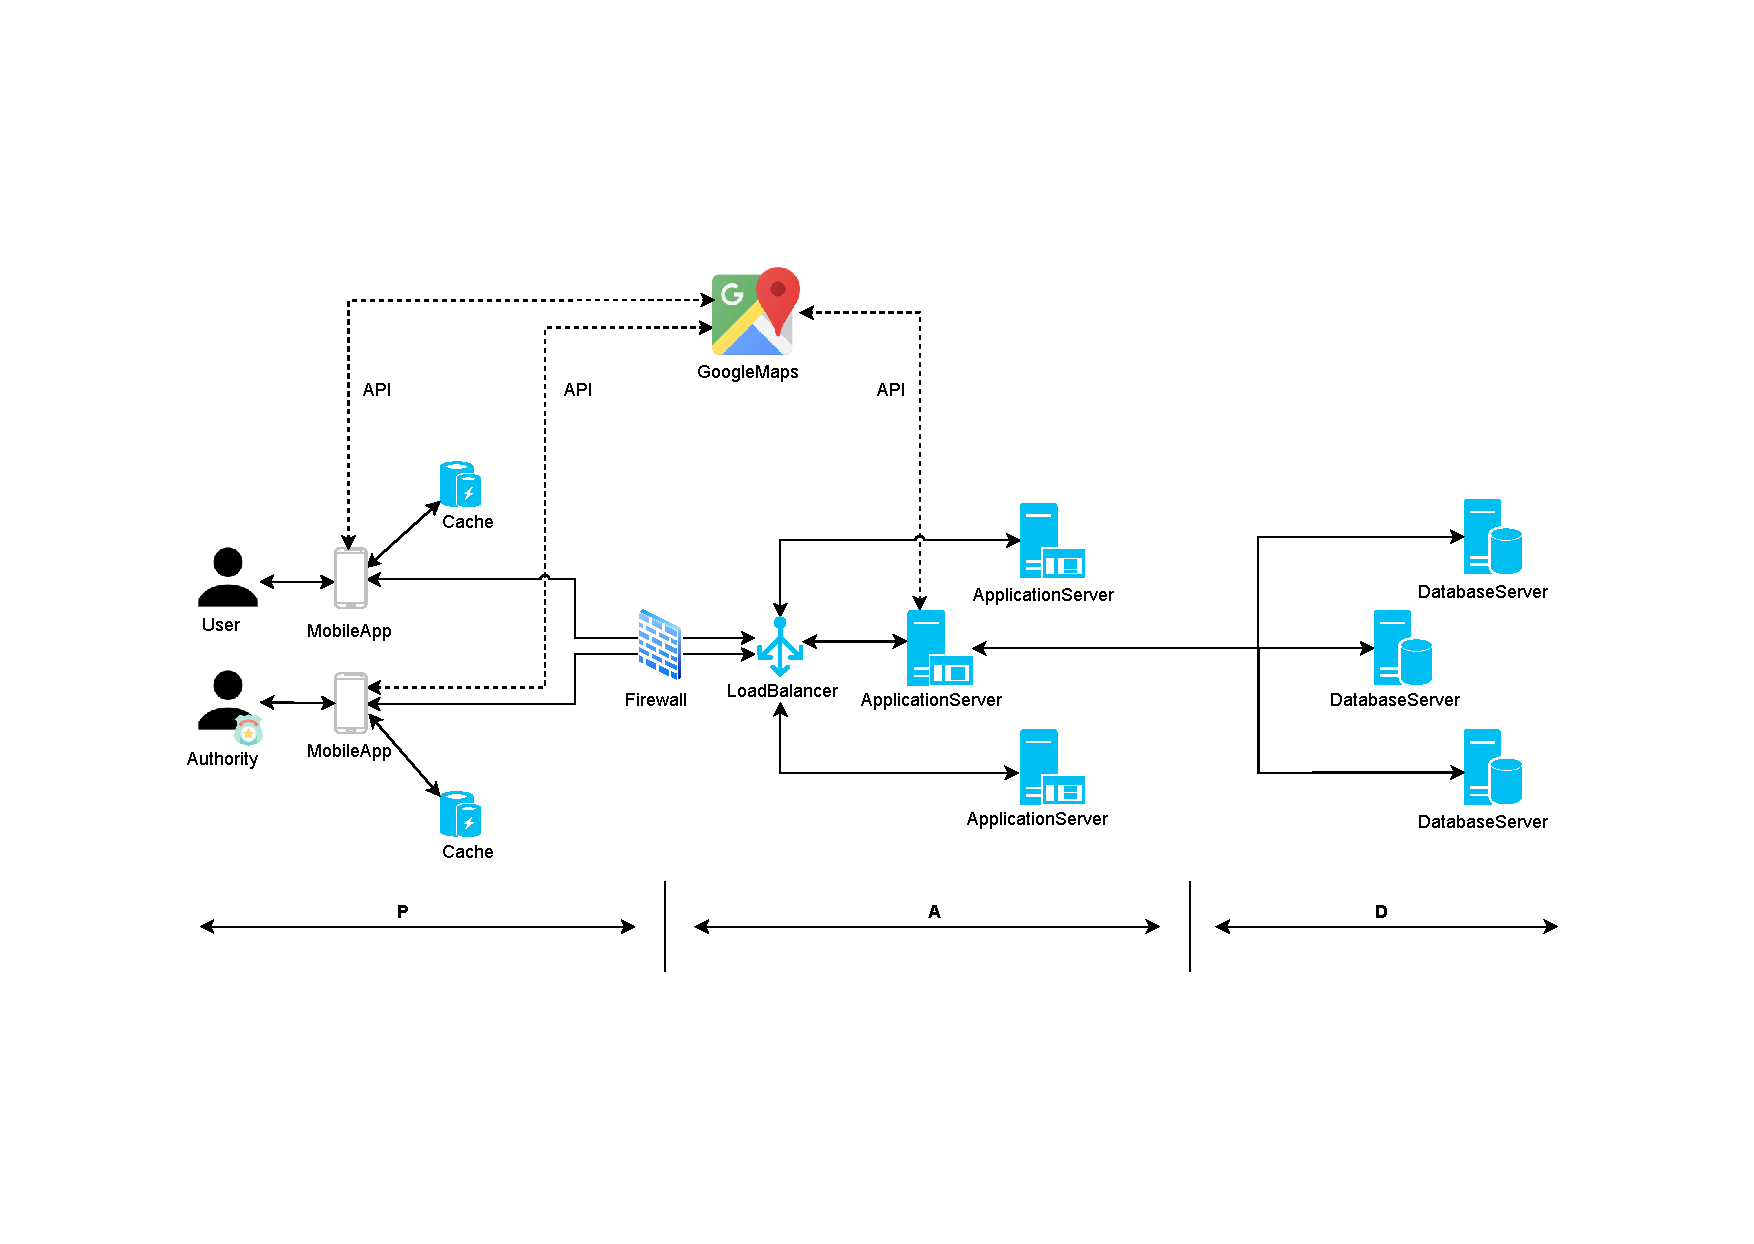
\includegraphics[scale = 0.6, center]{sysarch}
			\caption{System architecture}
	\end{figure}
	Users and authorities are provided with mobile devices and access the service through
	the SafeStreets mobile app. The mobile app communicates with the application layer, which
	is made by one or more application servers, linked to the database servers. The scale-out approach allows to adjust the number of hardware resources at any time. For what concerns the data access layer, database servers contain sensitive information, such as password hashes, license plate numbers, identification numbers and so on, so it is important to protect all the back-end of the application. In order to do this, the application and data access levels are protected by a firewall that performs traffic control at the level of the single packet, creating a DMZ in which the communication is safe. Another solution to reduce the computational load, as well as the messages, is the use of caches in the presentation tier: the mobile app stores on the mobile device memory part of the user's data, such as the sent reports and the results of reports evaluation, in order to make them available even when the users (or the authorities) have no access to Internet. This avoids many repeated requests for the same data, with heavy impact on the application and data acces layers' performance.
The system also includes a recommender system: exploiting data mining techniques, such as association rules, it can suggest to the authorities of one municipality possible interventions to improve security on the streets.

		\section{Component view}
		This section shows the internal composition of the application server, which is the core component of the system and contains the business logic,
		and its interaction with the external interfaces. In order to obtain a clear and understandable view, the system is described with three different diagrams,
		which contain the various components that communicate with a certain external component. The diagrams show the interaction of the application with the
		Google Maps APIs, the mobile application and the DBMS. After each diagram, a brief explanation of each component's role is provided, exception made for the 
		router, which is described before. Note that some managers can appear in more than on diagram, since they interact with more than one external
		interface.	
		
		\begin{itemize}
			\item\textbf{Router}: its role is to manage all the messages incoming from the other subsistems, forwording them to the right component and calling
			the appropriate method on it.
		\end{itemize}


	\begin{figure}[H]
				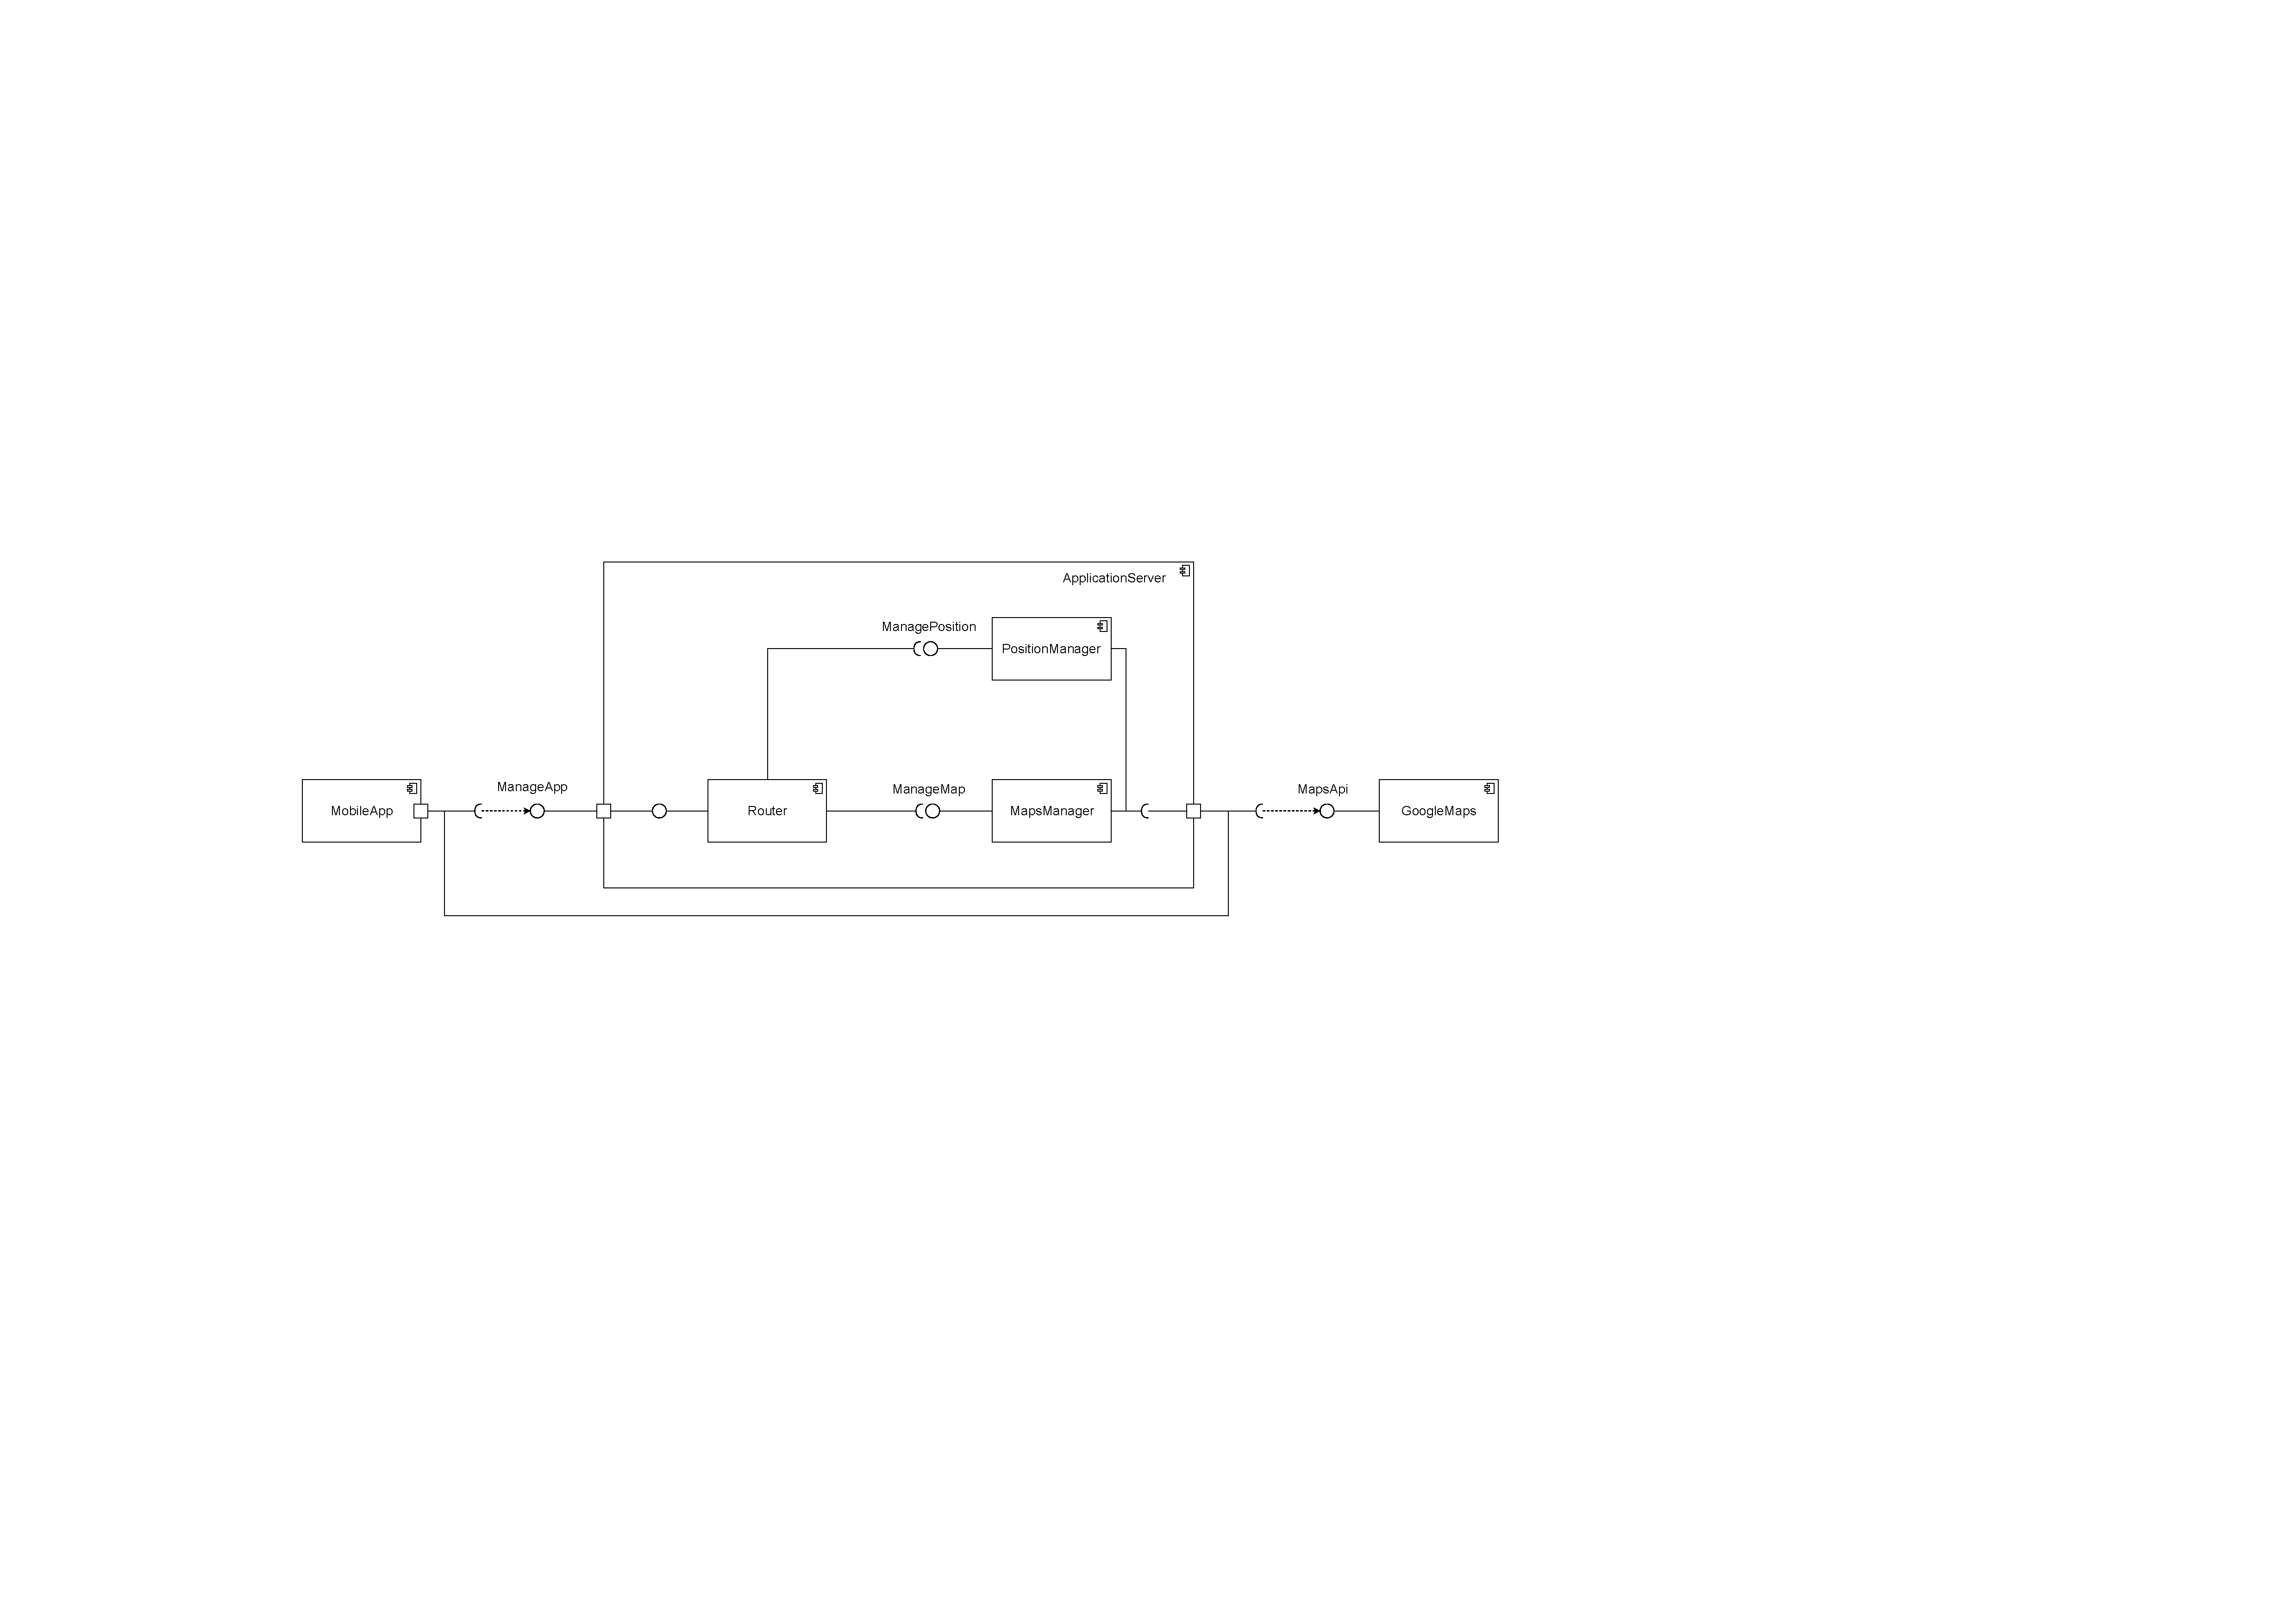
\includegraphics[scale = 0.4, center]{ComponentDiagramMaps}
				\caption{Component diagram - Google Maps}
	\end{figure}
		\begin{itemize}
			\item\textbf{PositionManager}: interacts with the client to retrieve the position of the user, then returns it to the caller.
			\item\textbf{MapsManager}: contains all the necessary methods to display the map of the violations and interact with it. Given a set of streets, 
			interacts with Google Maps APIs to obtain a map. 
		\end{itemize}
	
	\begin{figure}[H]
				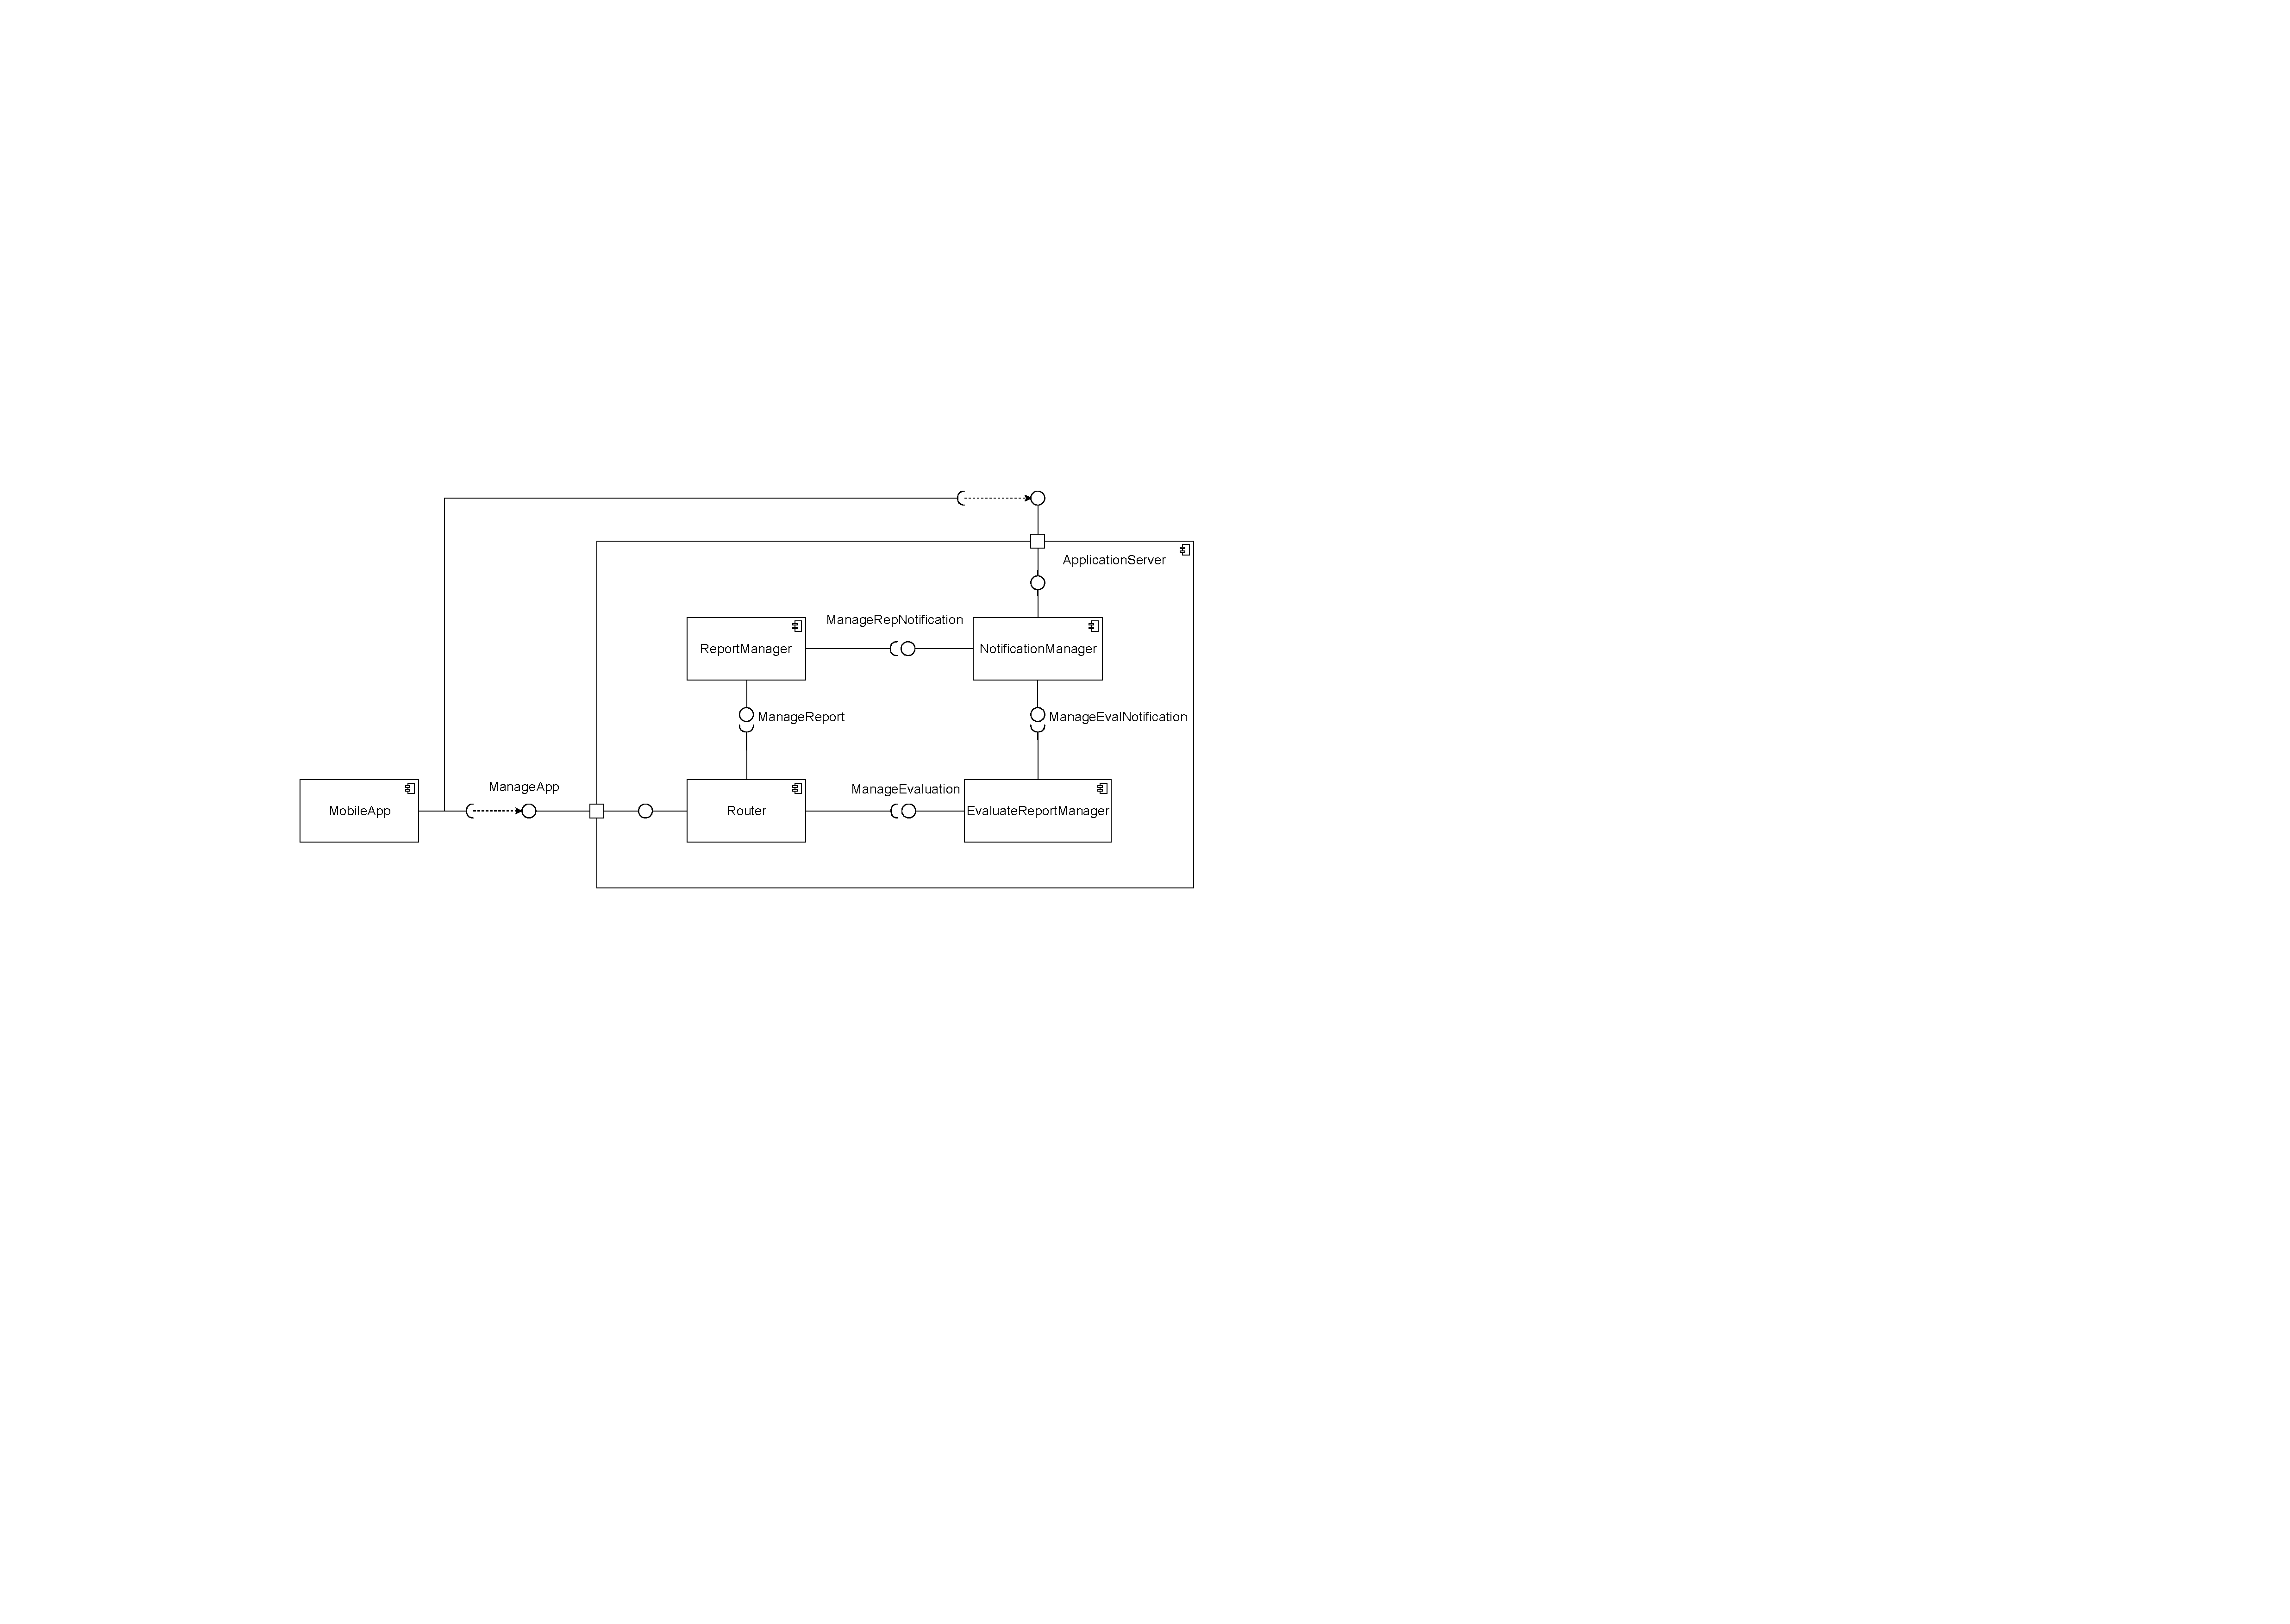
\includegraphics[scale = 0.5, center]{ComponentDiagramResponse}
				\caption{Component diagram - Response}
	\end{figure}
		\begin{itemize}
			\item\textbf{ReportManager}: manages the logic inherent the notification of the authorities, when a new report is available.
			\item\textbf{EvaluateReportManager}: as the ReportManager, but to notify users when one of their reports is evaluated.
			\item\textbf{NotificationManager}: manages the communication with the mobile application, to make sure that the messages are received correctly.
		\end{itemize}

	\begin{figure}[H]
				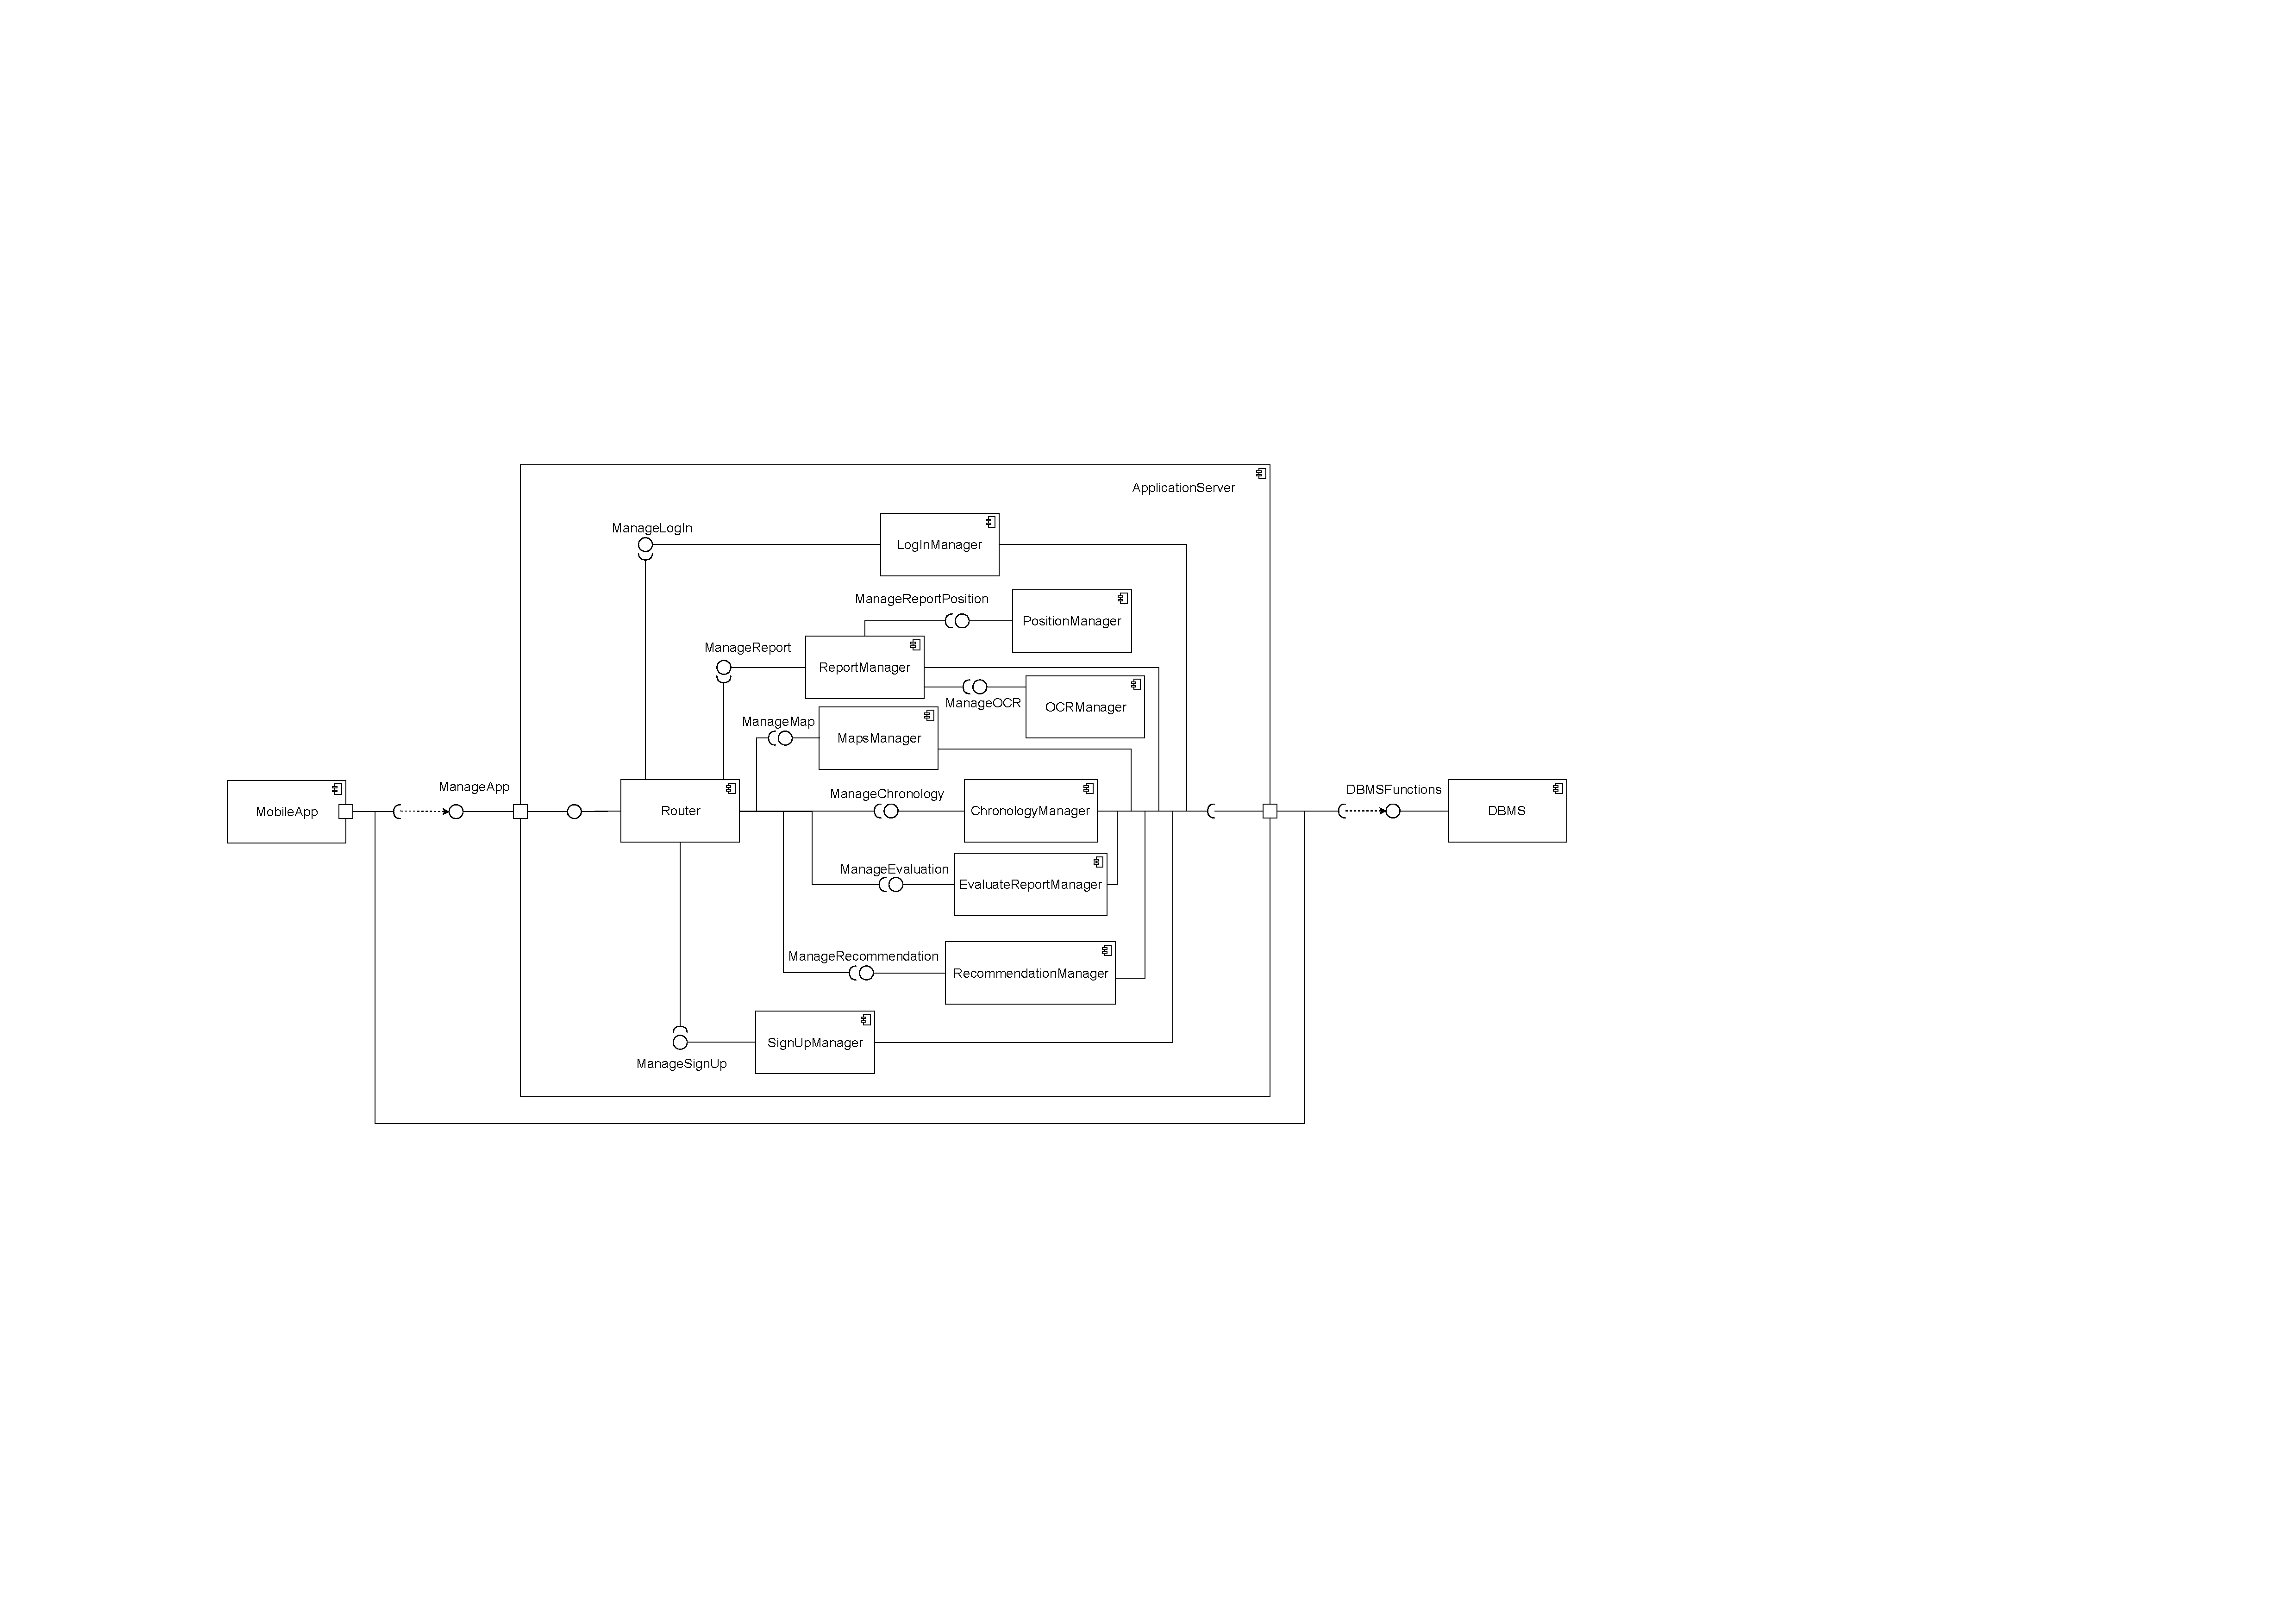
\includegraphics[scale = 0.4, center]{ComponentDiagramDBMS}
				\caption{Component diagram - DBMS}
	\end{figure}
		\begin{itemize}
			\item\textbf{SignUpManager}: handles the subscription process, both for users and authorities. Interacts with the DBMS to check if the provided
			credentials are already associated to other accounts.
			\item\textbf{LogInManager}: receives two strings, an e-mail address and a hash. Checks if the e-mail address is in the DBMS and if the password
			hashes match.
			\item\textbf{ReportManager}: contains all the logic necessary to complete a report: given all the information input by the user, completes it with
			the missing ones, like the user position and the license plate number.
			\item\textbf{PositionManager}: retrieves the device position to be attached to the report.
			\item\textbf{OCRManager}: given a pitcure, runs the OCR algorithm and returns a string. Notifies the PositionManager if, for any reason, the license
			plate number cannot be read.
			\item\textbf{MapsManager}: interacts with the DBMS, in order to retrieve the number and the type of reports for a given set of streets.
			\item\textbf{ChronologyManager}: when requested, obtains from the DBMS all the reports made by a given user and their status.
			\item\textbf{EvaluateReportManager}: stores in the DB the result of the evaluation of a report.
			\item\textbf{RecommendationManager}: implements the recommender system that periodically interacts with the DBMS, to check if some streets are
			involved in particular types of violation. In that case, it will suggest an intervention to the authorities of that municipality.
		\end{itemize}
		
		\section{Deployment view}
This section shows how the core functionalities of the system are developed on different devices, in other words,
how software artifacts are distributed on the deployment targets. 
	\begin{figure}[H]
			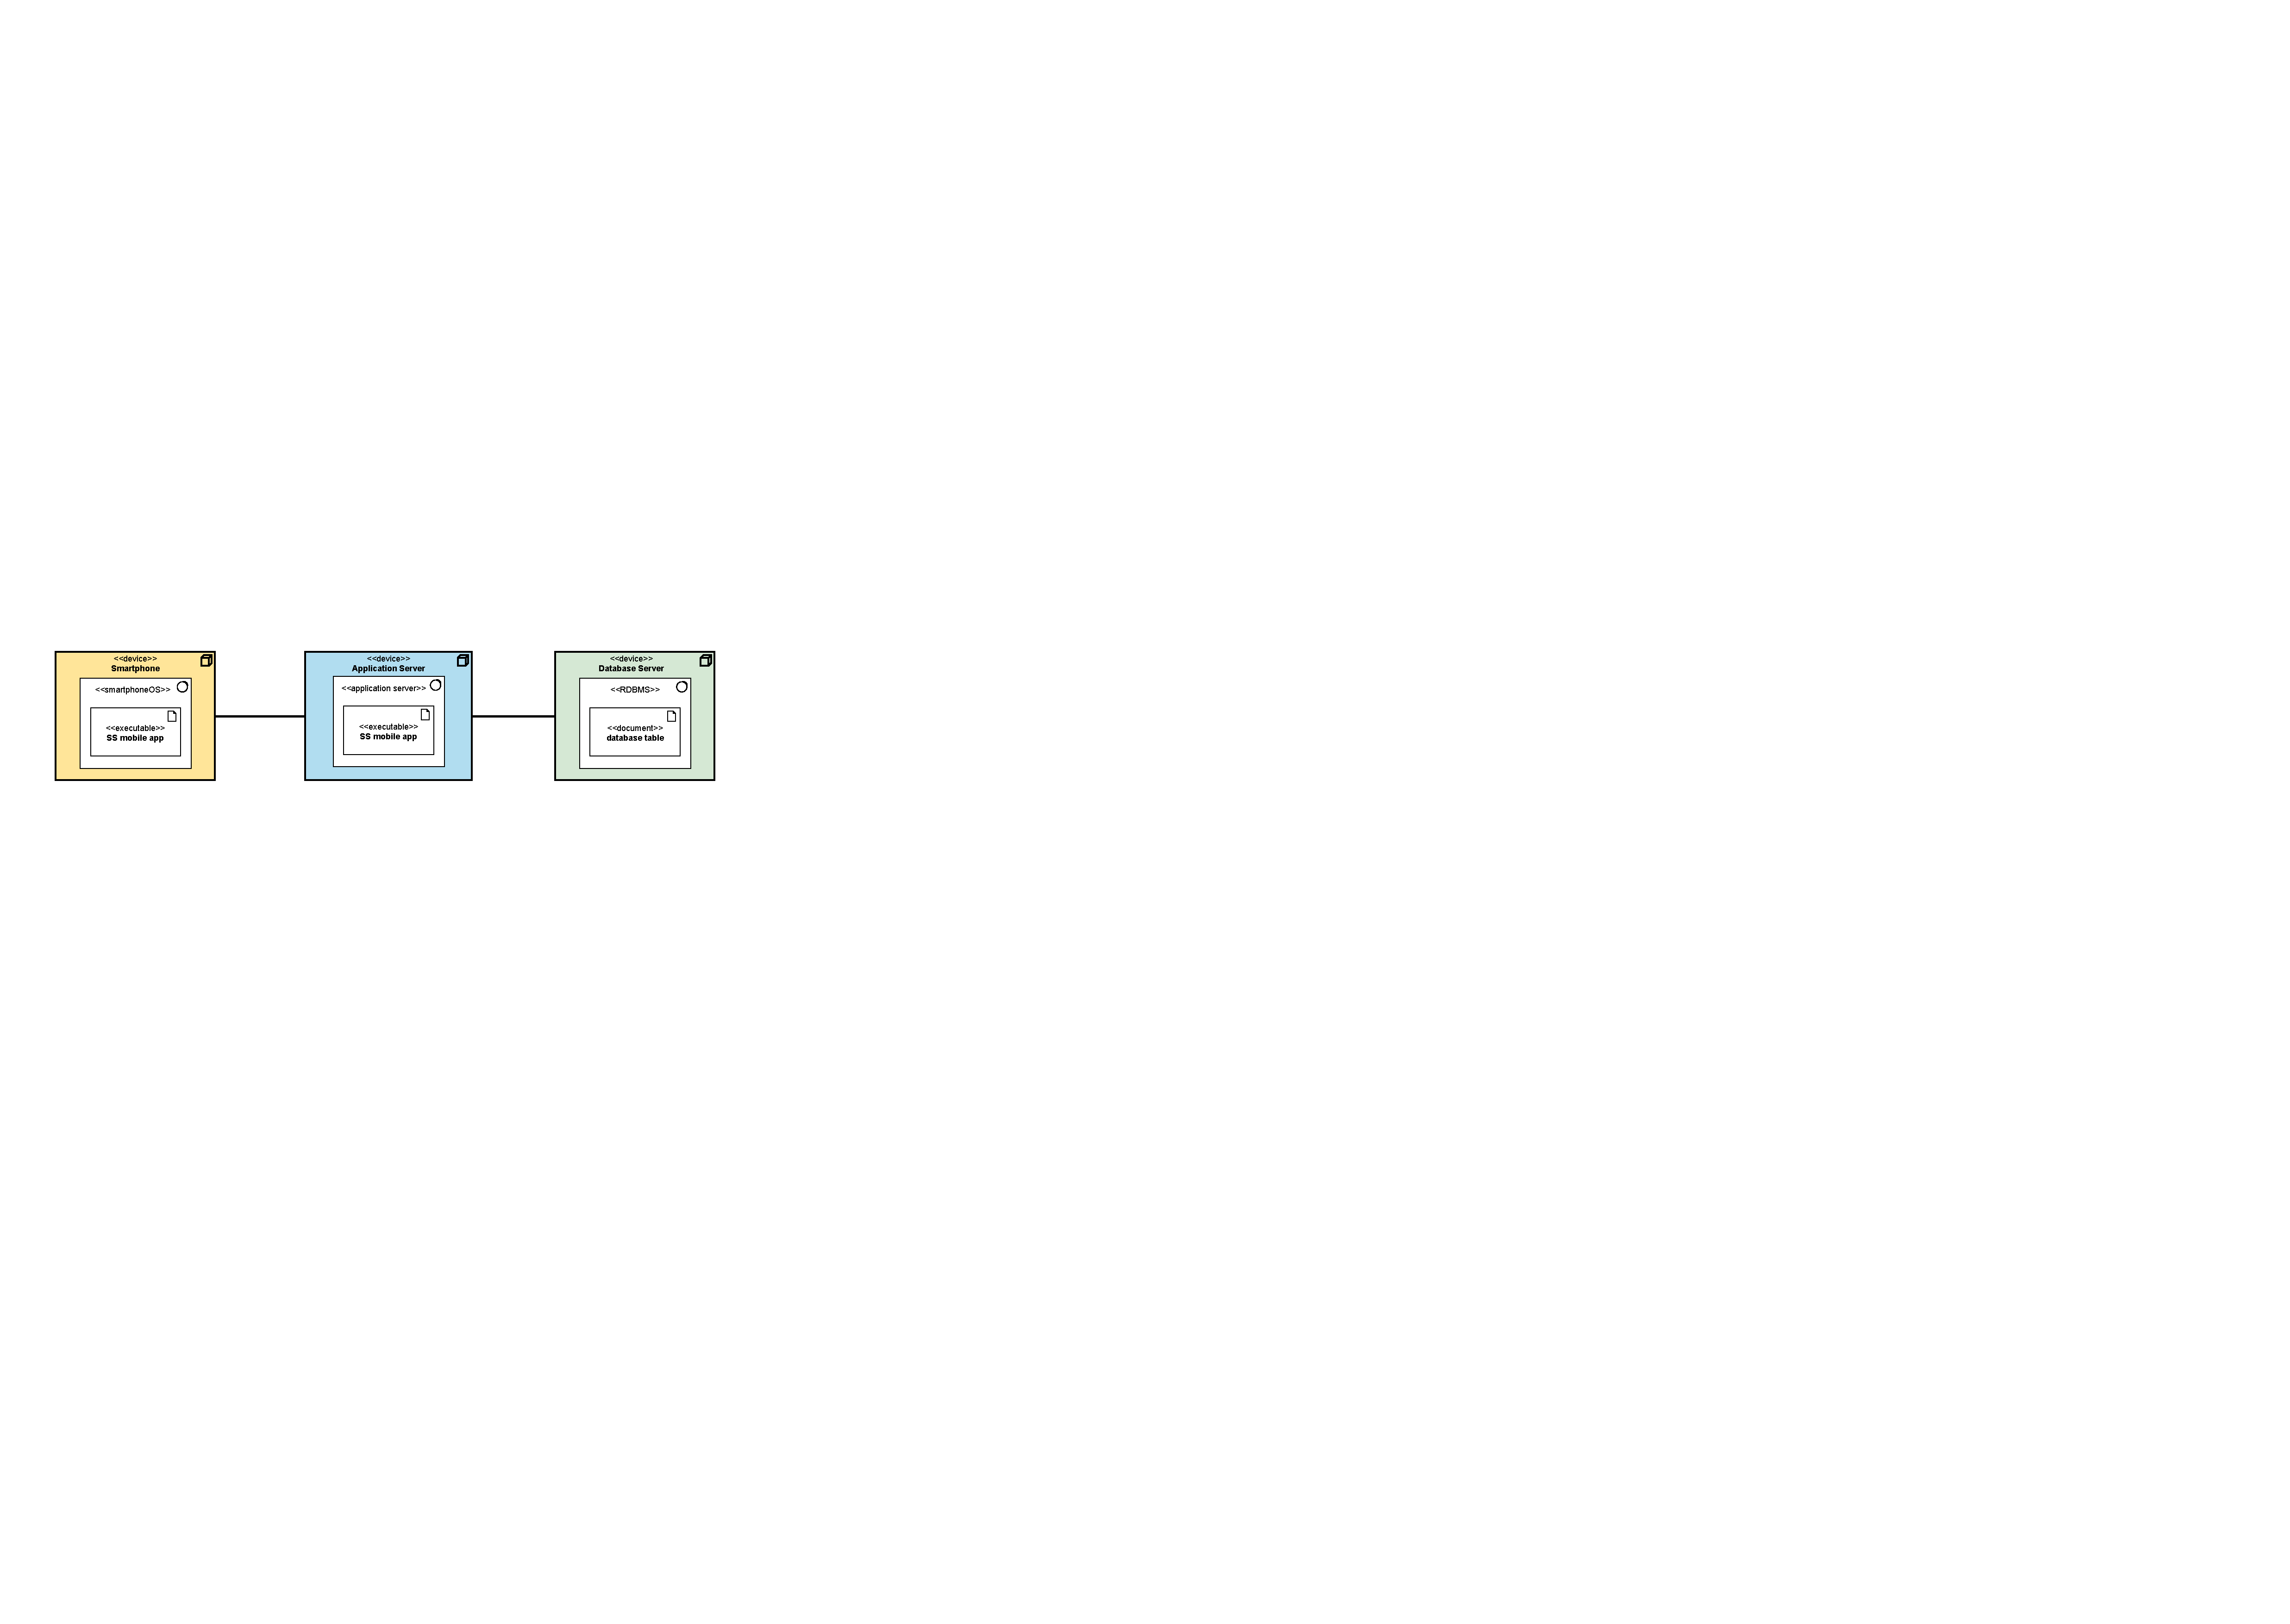
\includegraphics[scale = 0.6, center]{DeploymentDiagram}
			\caption{DeploymentDiagram}
	\end{figure}
The deployment diagram follows UML standard notation and does not represent external systems, like the load balancer and the firewall, in order to focus only on what must effectively be deployed on the three tiers:
\begin{itemize}
	\item\textbf{Tier 1}: hosts all the presentation logic. The mobile application must be developed for both iOS
and Android, to make it available for most of the devices. 
	\item\textbf{Tier 2}: here the application logic must be deployed. The application server communicates with both
the other tiers, handling all the requests.
	\item\textbf{Tier 3}: hosts the data access logic. The database server hosts a relational DBMS. The RDBMS is
preferred due to some reasons, like the possibility to use foreign keys in the tables or easily implement some rules
(like the one of requirement R13). With a future growth of data amount, a hybrid approach can be taken into account, for instance with the use of structured storage.
\end{itemize}

		\section{Runtime view}
			In this section will be presented the sequence diagrams of the various functionality, is up to the application
			controlling and guaranteeing that each user can access only to the right functionality.
			\subsection{Making report}
				\begin{figure}[H]
						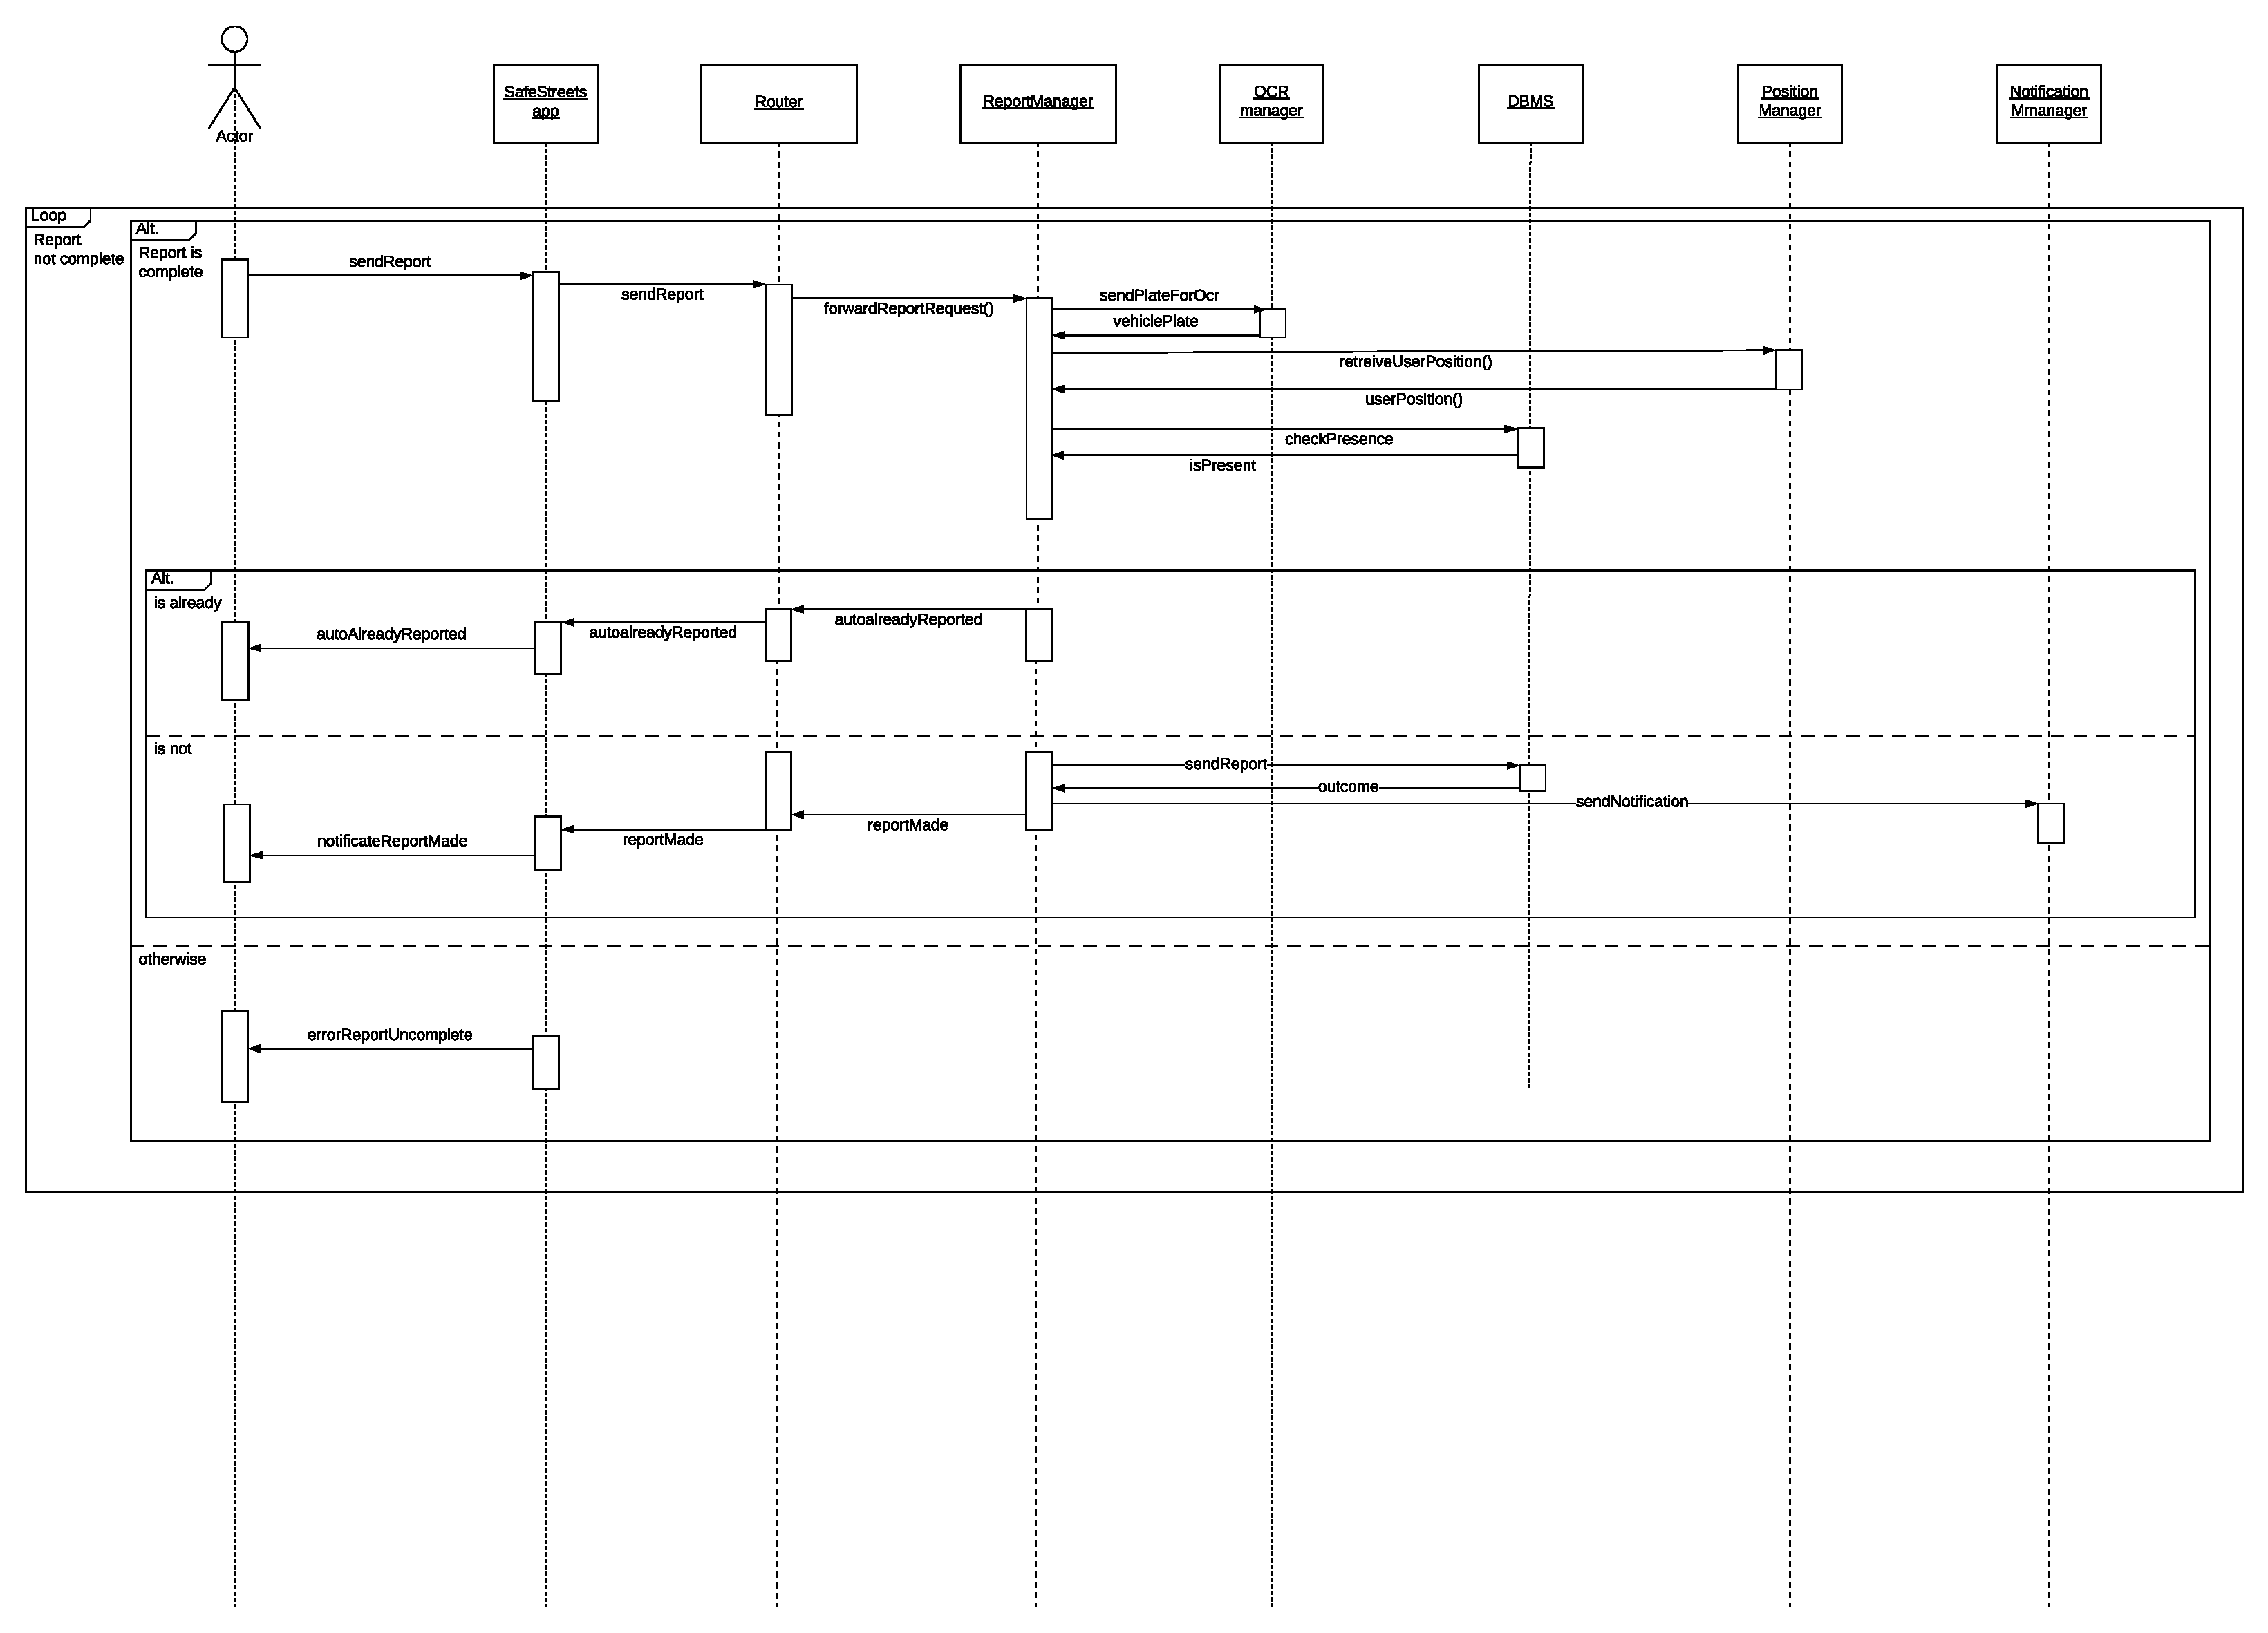
\includegraphics[width = 1.5\textwidth, center]{Report}
						\caption{How the report works}
						\label{fig: diagrams}
				\end{figure}
				This sequence diagrams explain the process through which a user can report a traffic violation.\\
				Once he has opened the application and logged in/signed up he can chose the ``Report violation" option,
				when he does that the application send the request to a router that forward the request to the right
				component (in this case the ``Report Manager").\\
				The first information the app request to the manager is to retrieve the user position, the request is forwarded
				to the Report manager and then to the Position manager (all request are centralized to the report manager).
				Then the user has to fill the form to report the traffic violations with the violation type and a photo of the
				violation and a photo of the plate. The request cannot be sent until all the form is completed.\\
				Is up to the application to verify that in the plate photo there is actually a plate. %How about that?
				Once the form has been sent the manager take care of the rest. First thing first the manager has to convert
				the photo of the plate into a String, so it send the plate's photo to the OCR manager, in this way using some
				photo manipulation techniques the system is able to obtain a String with the license plate.\\
				Once obtained that the report manager use a query to look up the database trying to find if there is already a
				pending (or resolved) report involving that car, in this way a car won't be reported twice for the same
				violations. If the vehicle has been already reported the application will display a message like ``I'm sorry but
				this vehicle has been already reported", to notify the user that the request failed.\\
				If it's not already reported the report is stored into the database, and a notification is sent to the authorities
				(using the notification manager).
			\subsection{Visualize Maps}
				\begin{figure}[H]
						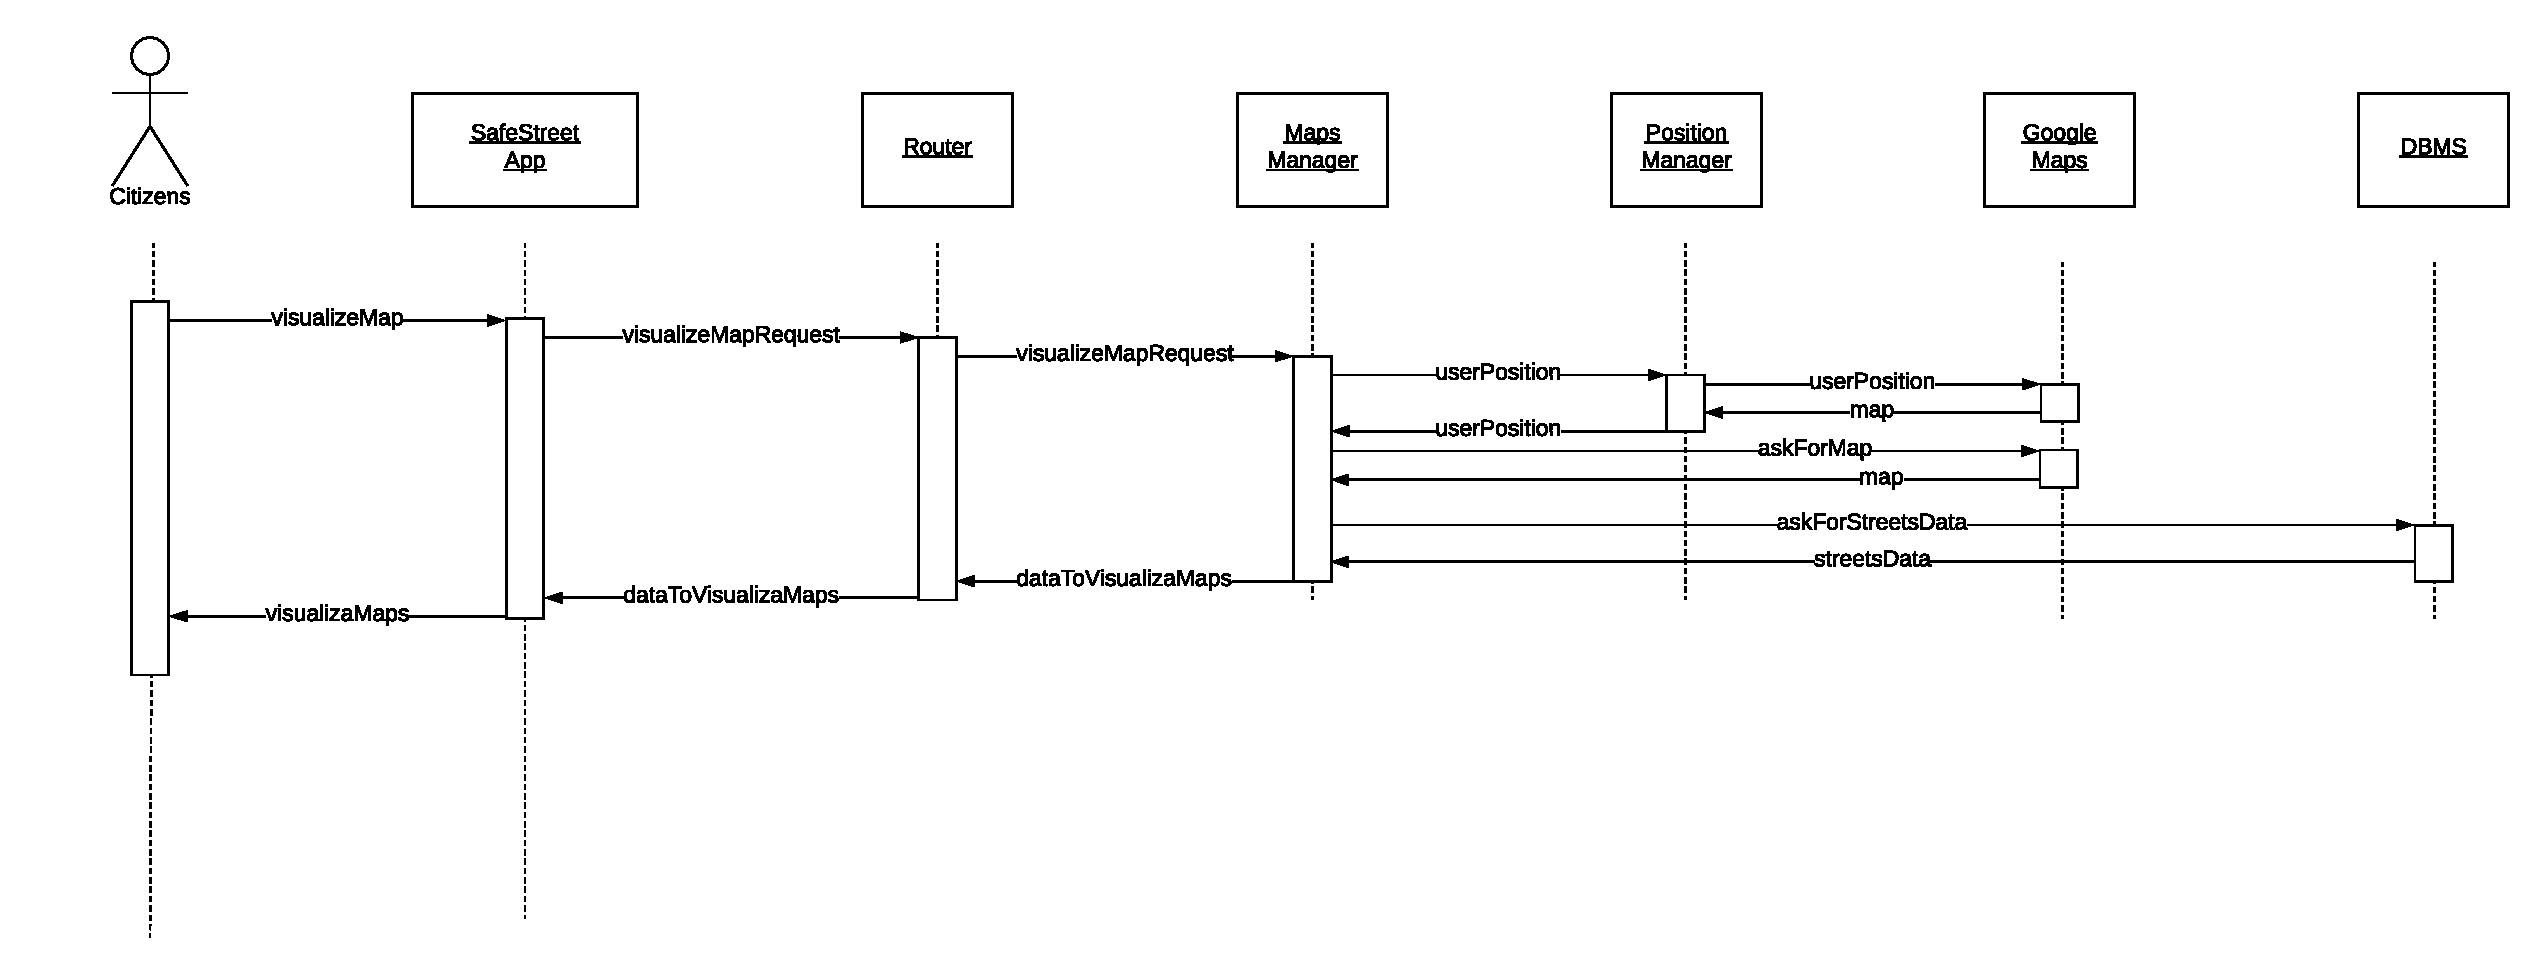
\includegraphics[width = \textwidth, center]{Maps}
						\caption{How map visualization works}
						\label{fig: diagrams}
				\end{figure}

				This sequence diagrams explain the process through which a user can visualize the map to indentify which
				streets have the highest number of violations.\\
				Once he has opened the application and logged in/signed up he can chose the ``Visualize map" option,
				when he does that the application send the request to a router that forward the request to the right
				component (in this case the ``Maps Manager").\\
				The manager take care of everything, it obtain the user position in order to load the correct map from google
				maps, then it contact the db to retrieve information about the streets in that map to apply the correct colors
				and in the end it sends all to the application.
			\subsection{Visualize reports' history}
				\begin{figure}[H]
						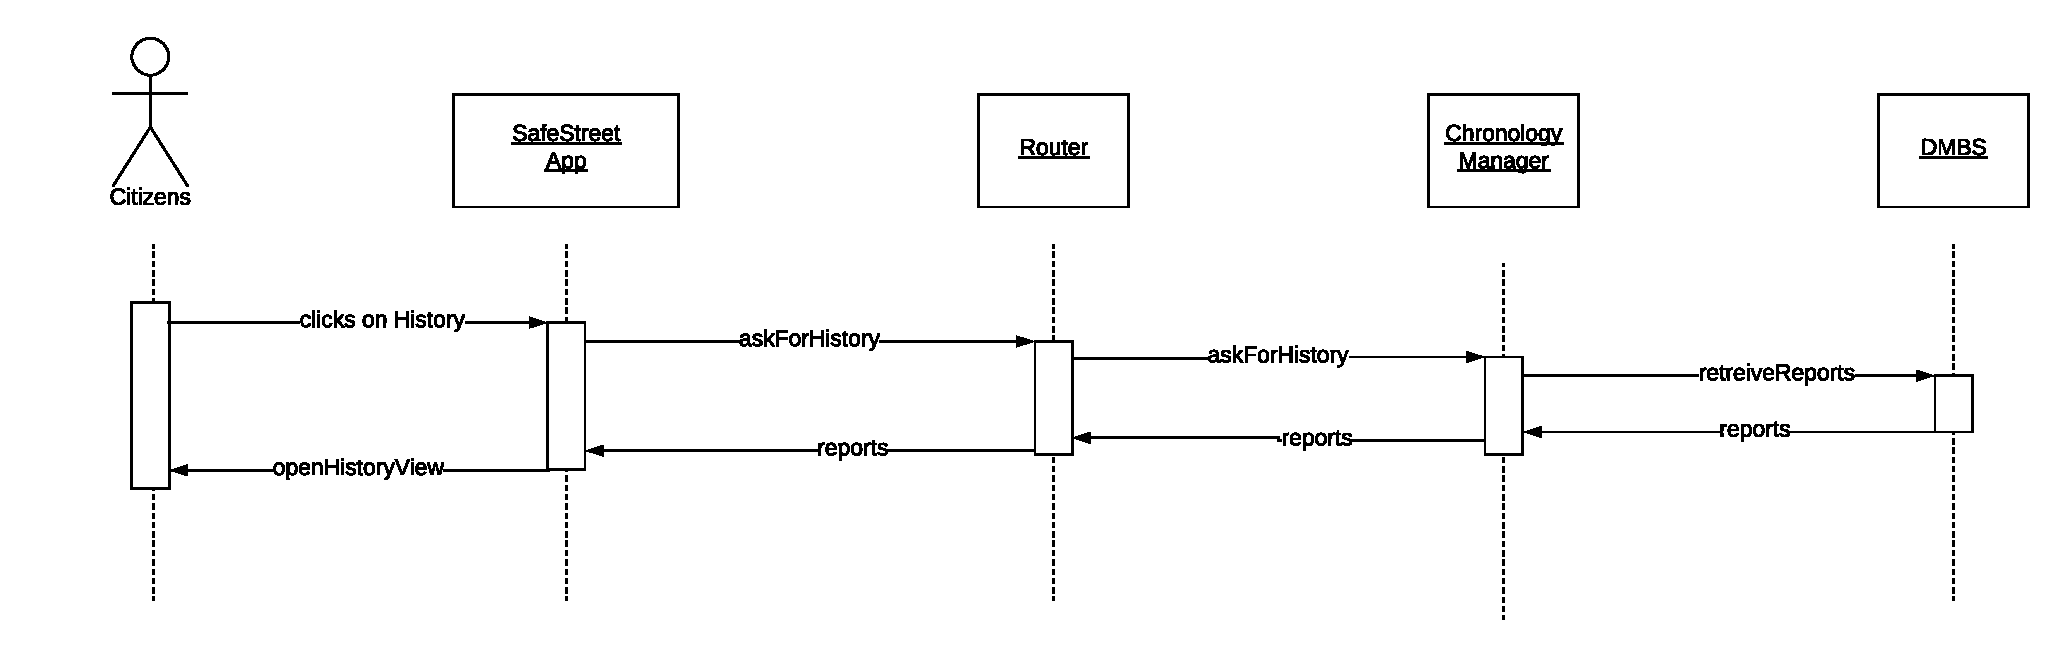
\includegraphics[width = \textwidth, center]{history}
						\caption{How reports' history works}
						\label{fig: diagrams}
				\end{figure}
				This sequence diagrams explain the process through which a user can visualize the history of his previous
				reports.\\
				Once he has opened the application and logged in/signed up he can chose the ``My reports" option,
				when he does that the application send the request to a router that forward the request to the right
				component (in this case the ``Chronology Manager").\\
				The manager simply obtains all the previous reports by querying the db, if there aren't reports the manager
				will send a message to the app and will be displayed something like ``I am sorry, it seems that you didn't any
				report up to now".
				The user will see date\&time of each report, the status (pending, approved or rejected), the street and the
				type of violation.\\
				The plate won't be displayed to protect the privacy of the other citizens.
			\subsection{Evaluate report}
				\begin{figure}[H]
						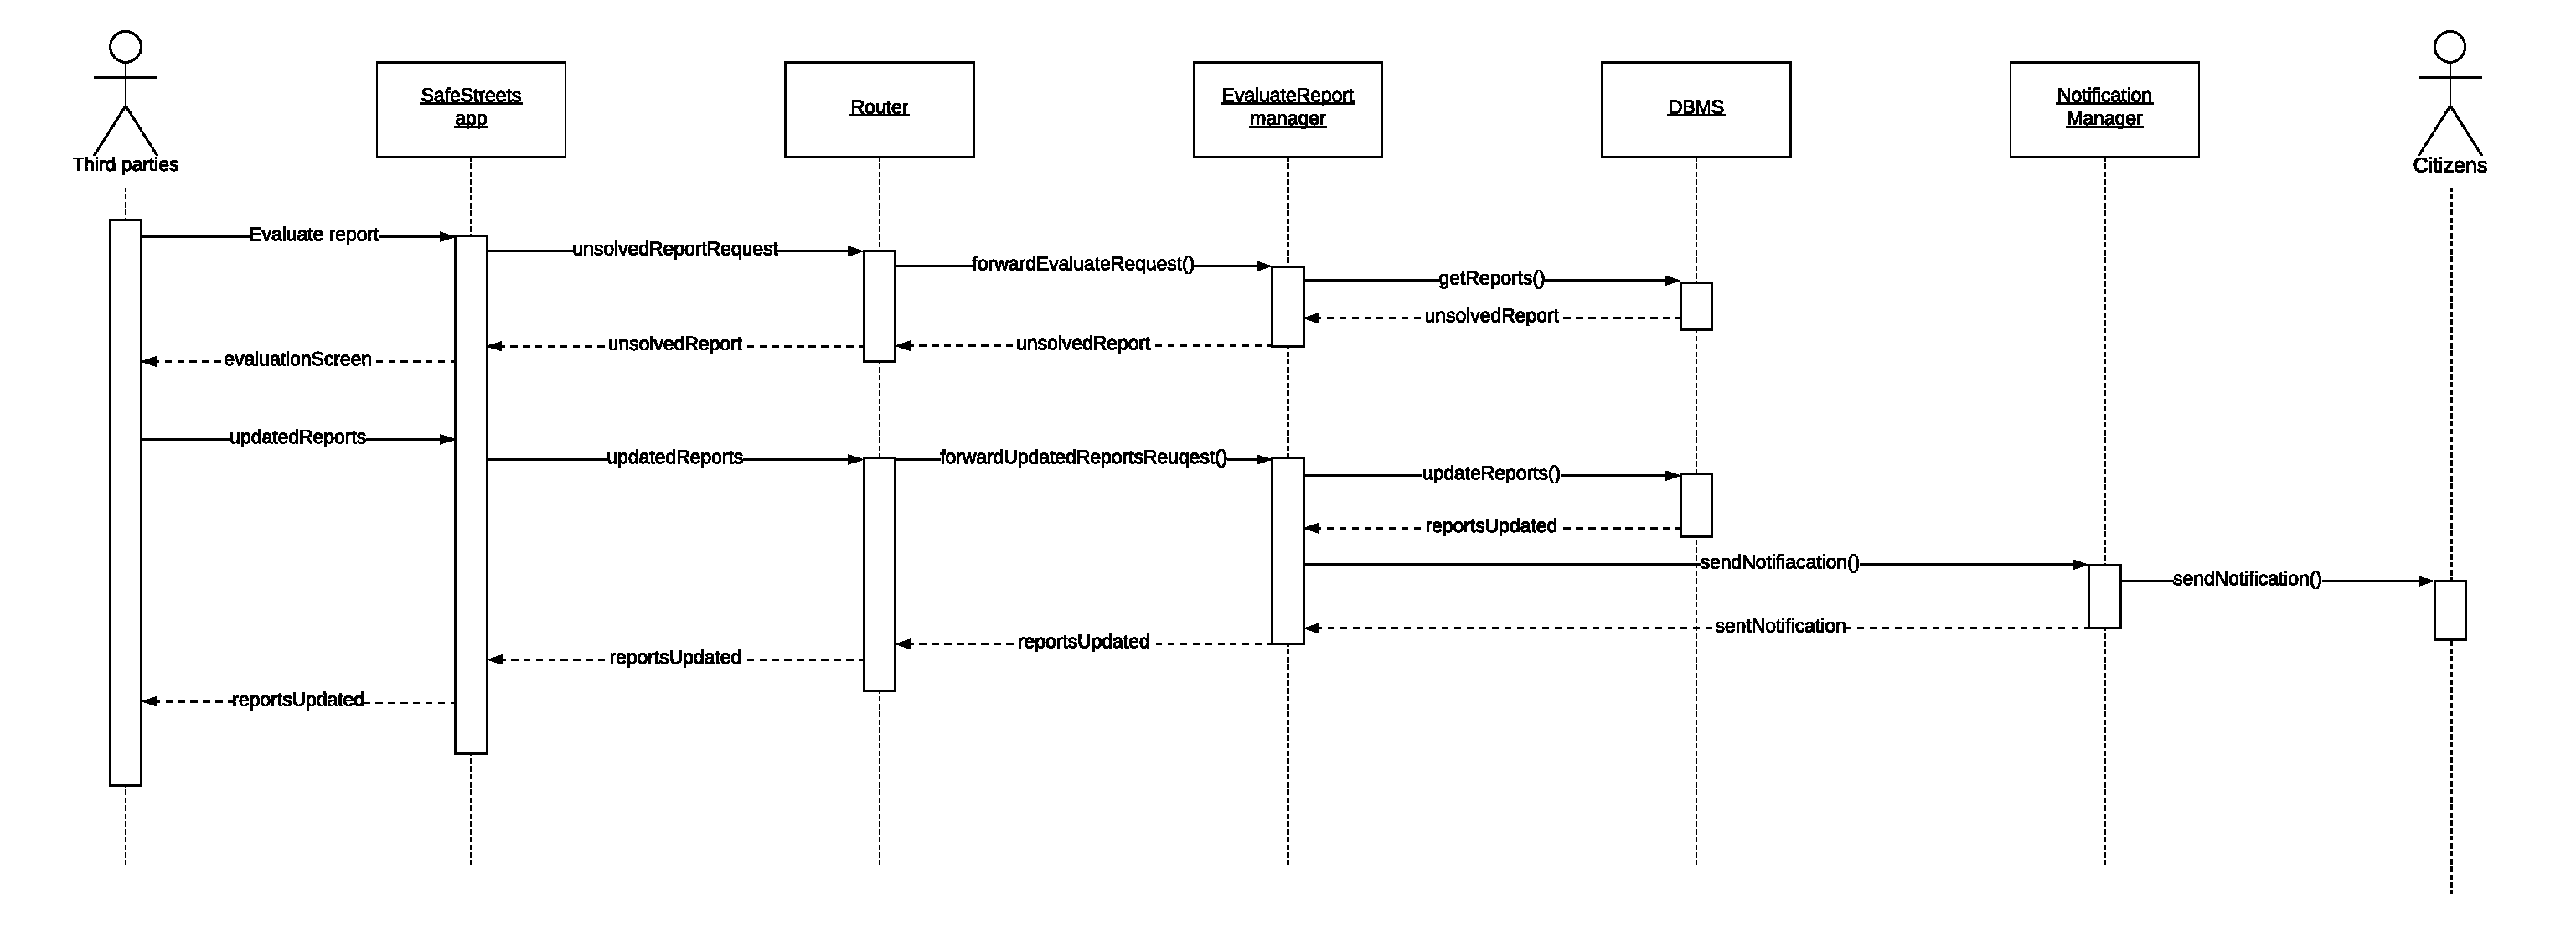
\includegraphics[width = \textwidth, center]{Evaluate}
						\caption{How reports are evaluated}
						\label{fig: diagrams}
				\end{figure}
				This sequence diagrams explain the process through which an authorities can evaluate pending reports.\\
				Once he has opened the application and logged in/signed up he can chose the ``Evaluate" option,
				when he does that the application send the request to a router that forward the request to the right
				component (in this case the ``Evaluation Manager").\\
				The manager retrieve from the db all the unsolved reports and send them to the application module, each
				time that an authority resolve a report the manager update the db and, using the notification manager, send
				a notification to the user who made it to notify him the updated status.
			\subsection{Asking for recommendation}
				\begin{figure}[H]
						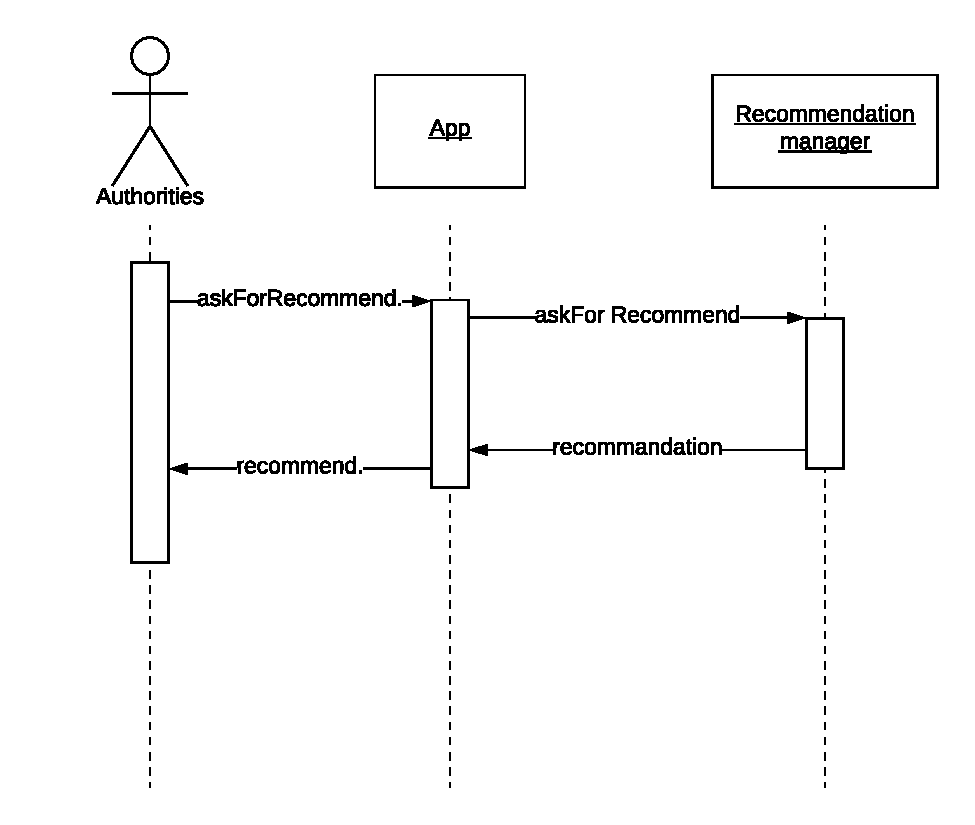
\includegraphics[width = \textwidth, center]{recommendation}
						\caption{How reports are evaluated}
						\label{fig: diagrams}
				\end{figure}
				This sequence diagrams explain the process through which an authorities can receive suggestion to improve
				the safety on the streets.\\
				Once he has opened the application and logged in/signed up he can chose the ``Recommend" option,
				when he does that the application send the request to a router that forward the request to the right
				component (in this case the ``Recommendation Manager").\\
				To receive recommendation on how to improve the safety on the streets the manager will use a recommender
				system based on content base approach based on item content matrix. To receive suggestion the manager
				will consult the recommender system and obtain the best possible solution, then it will be forwarded to the
				application.
		\section{Component interfaces}
			\subsection{Overall summary}
				In this section will be analyzed the interfaces necessary to each function, explaining the purpose of the main
				functions.
			\subsection{Main page}
				\begin{figure}[H]
						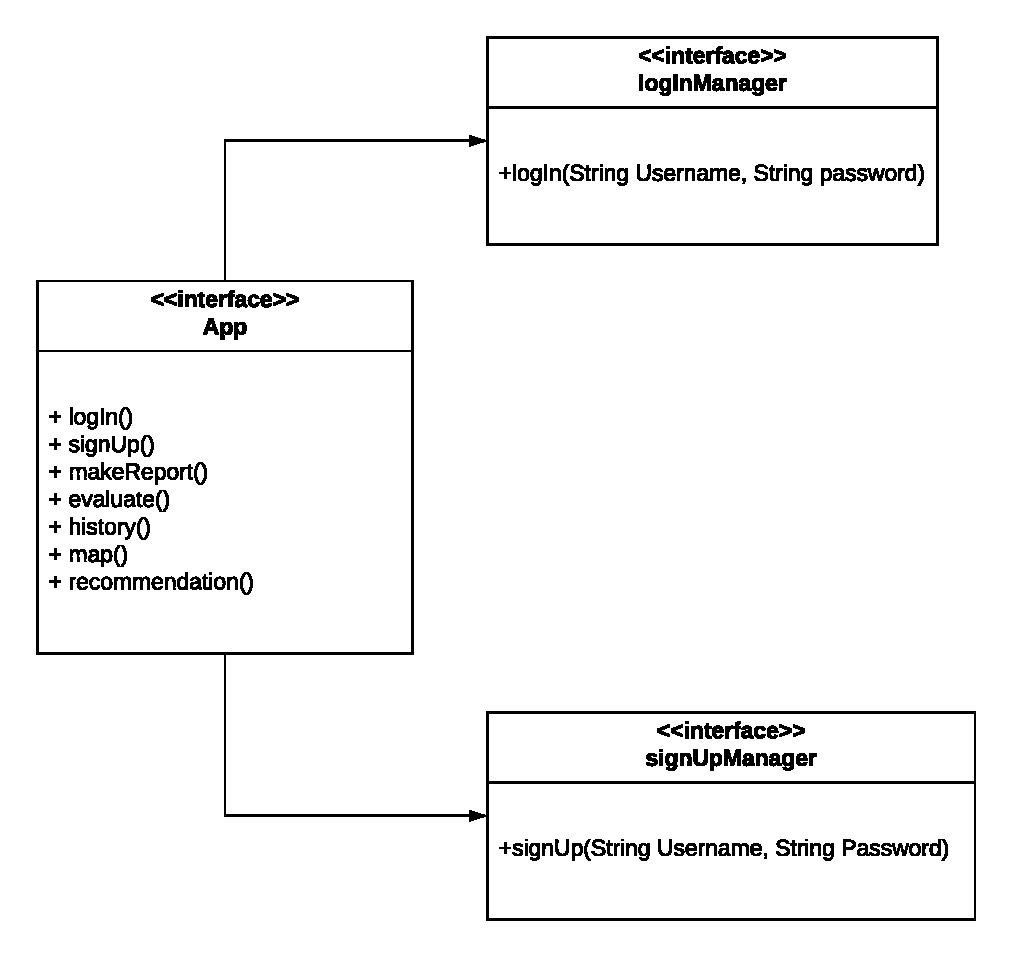
\includegraphics[width = \textwidth, center]{mainInterface}
						\label{fig: interfaces}
				\end{figure}
				\newpage In the figure above is represented the interface to manage the main page of the application.
				It is important to underline that it is the task of the application to ensure that each user can access the
				functions dedicated to him and not to others (for example a citizen can't see the evaluate option).
				%Is also up
				%to the system to check the validity of the created reports.
				%Here a quick description of the functions illustrated above:
					\begin{itemize}
						\item \textbf{App}
						\begin{itemize}
							\item \textbf{logIn} This method obtain the information from the ``Username" and the
								``Password" fields, and then call the logInManager
							\item \textbf{signUP} This method display the sign up form, then it obtain all the data
								from the fields and it controls their validity, then to complete the procedure and
								save the user in the db it calls the method ``sign up" from  ``sign up manager"
							\item \textbf{makeReport} This method display the form to report traffic violations and
								it starts the procedure, it will call all the methods of ``reportManager"
								(will be explained in detail to follow). 
							\item \textbf{evaluate} This method display the screen to evaluate traffic violations and
								it starts the procedure, it will call all the methods of ``evaluateManager"
								(will be explained in detail to follow).
							\item \textbf{history} This method display the history of the user's reported traffic
								violations and it starts the procedure, it will call all the methods of
								``historyManager" (will be explained in detail to follow).
							\item \textbf{map} This method display the map with the streets colored in function of the
								traffic violations' number.
							\item \textbf{recommendation} This method will give a suggestion on how to improve the
								safety on a particular street, the methods involved will be explained in detail to
								follow in the  ``recommendationManager".
						\end{itemize}
						\item \textbf{signUpManager}
						\begin{itemize}
							\item \textbf{signUp} This method will communicate in a safe way to the DB using an
								asymmetric key, it will memorize into the DB the Username and the hash of the
								password.
						\end{itemize}
						\item \textbf{logInManager}
						\begin{itemize}
							\item \textbf{logIn} This method will communicate in a safe way to the DB using
								symmetric encryption (established at the begging of the communication using
								asymmetric encryption), it will obtain the password's hash from the DB and it will
								confront it to the hash of the one the user inserted.
						\end{itemize}
					\end{itemize}
			\subsection{Report}
				\begin{figure}[H]
						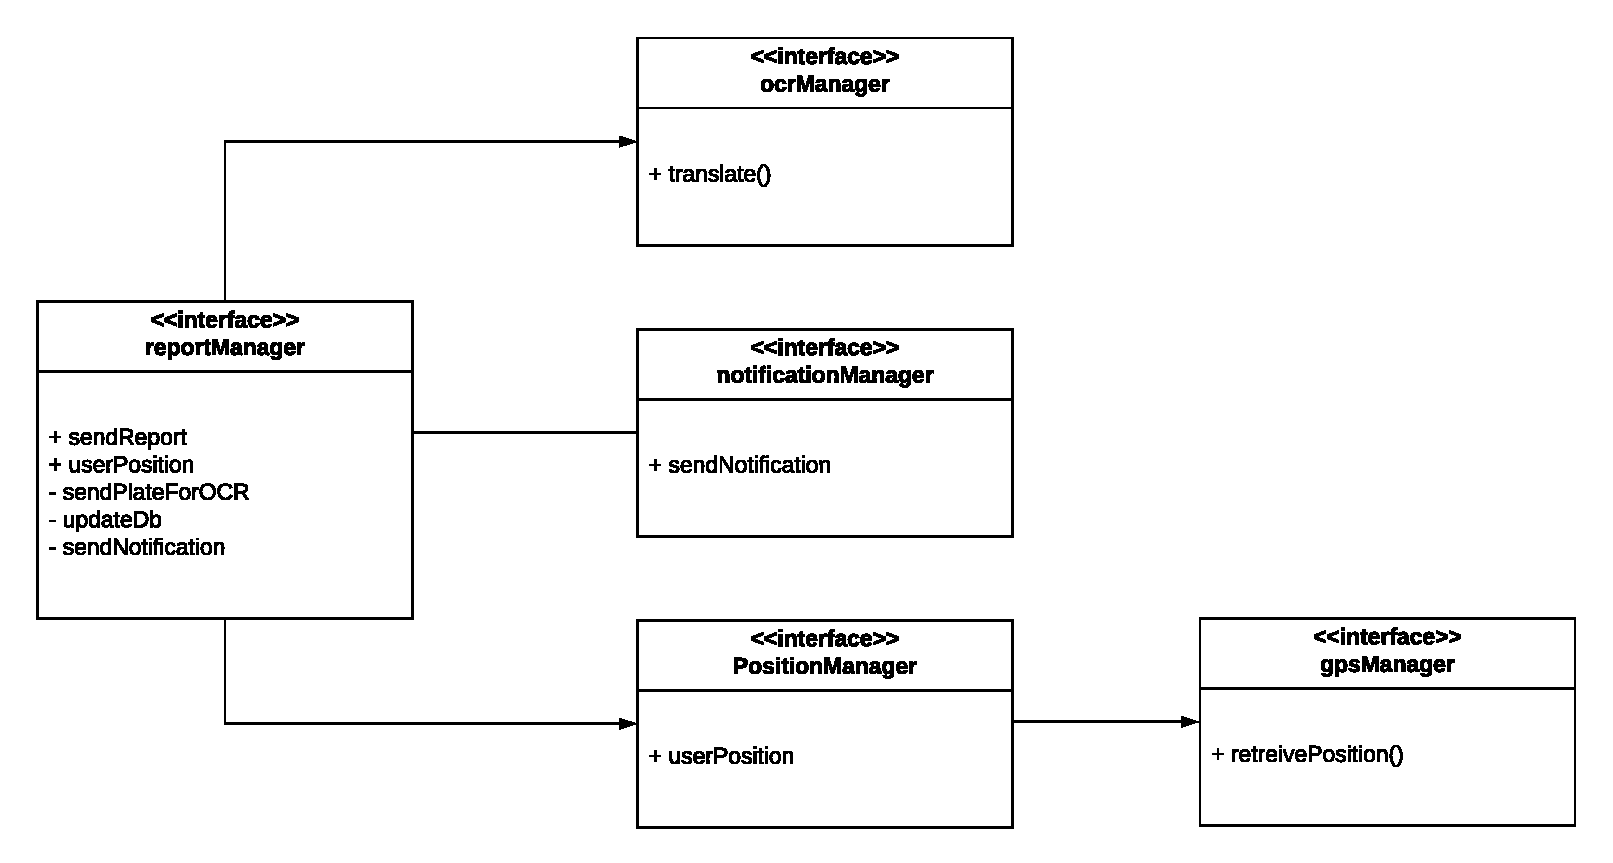
\includegraphics[width = \textwidth, center]{reportInterface}
						%\caption{How reports are evaluated}
						\label{fig: interfaces}
				\end{figure}
				\begin{itemize}
					\item \textbf{reportManager}
					\begin{itemize}
						\item \textbf{sendReport} This method take the created reports and save it onto the DB adding
						the status (pending), and the username who created it.
						\item \textbf{userPosition} This method contact the position manager to retrieve the user
						position and send it to the client to include it in the report.
						\item \textbf{sendPlateForOCR} This method is called by the client, is used to translate the
						plate's photo into a String to include it into the DB and facilitate further operation of query
						\item \textbf{updateDb} This is the method that take care of every communication with the DB.
						\item \textbf{sendNotification} This method is used to notify the authorities of new reports.
					\end{itemize}
					\item \textbf{ocrManager}
					\begin{itemize}
						\item \textbf{translate} This is the method that using OCR techniques obtain the license plate
						from the photo.
					\end{itemize}
					\newpage \item \textbf{notificationManager}
					\begin{itemize}
						\item \textbf{sendNotification}  This method is up to contact the users required (both citizens
						and authorities) to notify them new reports (or updated status of previous ones).
					\end{itemize}
					\item \textbf{positionManager}
					\begin{itemize}
						\item \textbf{userPosition} This method is up to retrieve the user position using some techniques
						(not only using the GPS system but also using mobile data or wi-fi)
					\end{itemize}
					\item \textbf{gpsManager}
					\begin{itemize}
						\item \textbf{retreivePosition} This method is specific to retrieve the user position using only the
							GPS system.
					\end{itemize}
				\end{itemize}
			\subsection{History}
				\begin{figure}[H]
						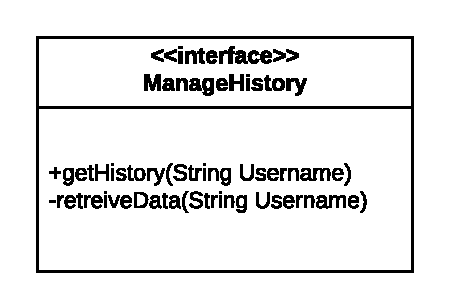
\includegraphics[center]{historyInterface}
						%\caption{How reports are evaluated}
						\label{fig: interfaces}
				\end{figure}
				\begin{itemize}
					\item \textbf{getHistory} This method has to communicate with the application, receiving requests and
						sending back the data.
					\item \textbf{retreiveData} This method is specific to contact and query the DB to obtain the history of
						user's reports. 
				\end{itemize}
			\subsection{Map}
				\begin{figure}[H]
						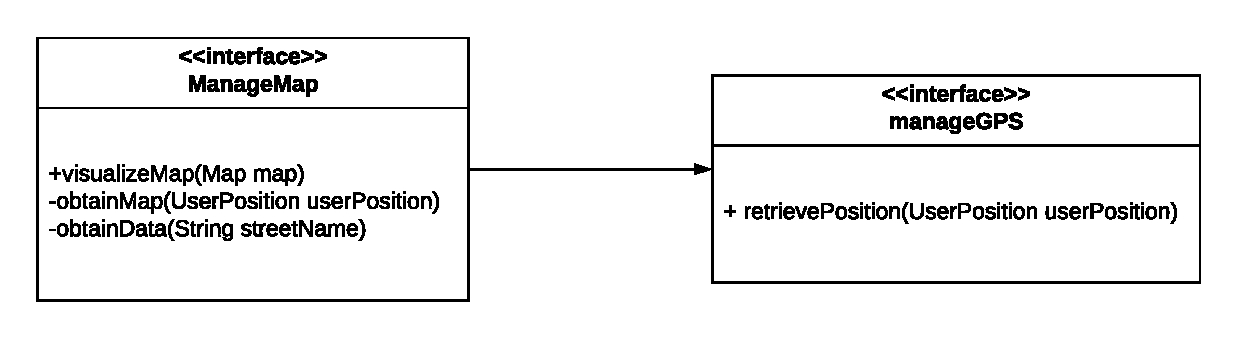
\includegraphics[width = \textwidth, center]{mapInterface}
						%\caption{How reports are evaluated}
						\label{fig: interfaces}
				\end{figure}
				\begin{itemize}
						\item \textbf{mapManager}
						\begin{itemize}
							\item \textbf{visualizeMap} The method retrieve the data about reports and the streets
								and then combine it assigning each street the right color. 
							\item \textbf{obtainMap} Is called by visualizeMap and contact the gpsManager to
								retrieve the user position and then google Map to obtain the map around him.
							\item \textbf{obtainData} Is called by visualizeMap and this method has to contact the DB
								and it has to obtain the number of reports in each street visualized on the map in
								order to make able visualizeMap to coloring it correctly.
						\end{itemize}
						\item \textbf{gpsManager}
						\begin{itemize}
							\item \textbf{retreivePosition} Same as said above (in report).
						\end{itemize}
				\end{itemize}
			\subsection{Evaluate}
				\begin{figure}[H]
						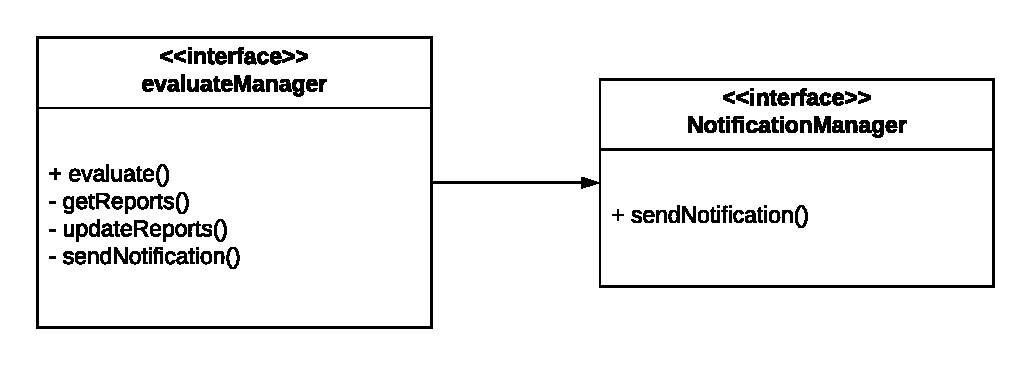
\includegraphics[width = \textwidth, center]{evaluateInterface}
						%\caption{How reports are evaluated}
						\label{fig: interfaces}
				\end{figure}
				\begin{itemize}
						\item \textbf{evaluateManager}
						\begin{itemize}
							\item \textbf{evaluate:} Communicate with the client sending the pending reports and
								receiving all updated reports.
							\item \textbf{getReports:} This method is called by evaluate and obtain all pending
								reports in the area under the jurisdiction of the authority who made the request.
							\item \textbf{updateDB:} This method is called by evaluate and updates the DB with the
								new status of the evaluated reports
							\item \textbf{sendNotification:} allert the user which report has been evaluated
						\end{itemize}
						\item \textbf{notificationManager}
						\begin{itemize}
							\item \textbf{sendNotification:} as said above
						\end{itemize}
				\end{itemize}
			\subsection{Suggestion}
				\begin{figure}[H]
						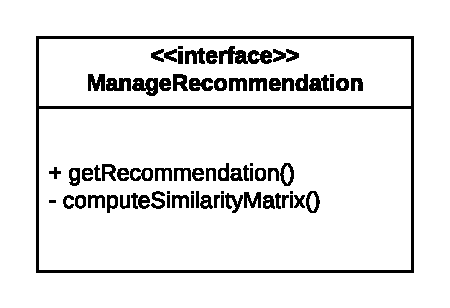
\includegraphics [center]{recommendationInterface}
						%\caption{How reports are evaluated}
						\label{fig: interfaces}
				\end{figure}
				\begin{itemize}
					\item \textbf{getRecommendation} This method receive the request and, with the matrix already
						compiled it take the 3 most similar recommendation made by the system and forward them to the
						authority.
					\item \textbf{computeSimilarityMatrix} This method is used each time some data are added, it compute
					the similarity matrix between the most frequent problem (each problem is divided in small aspect and
					each of them is an attribute) and a ICM where each item is a possible solution (the attributes are some
					aspect of the problems that each solution can resolve)
				\end{itemize}
	
	\subsection{Class diagram}
	As in the RASD, the following UML diagram describes the organization of the model.

		\begin{figure}[H]
				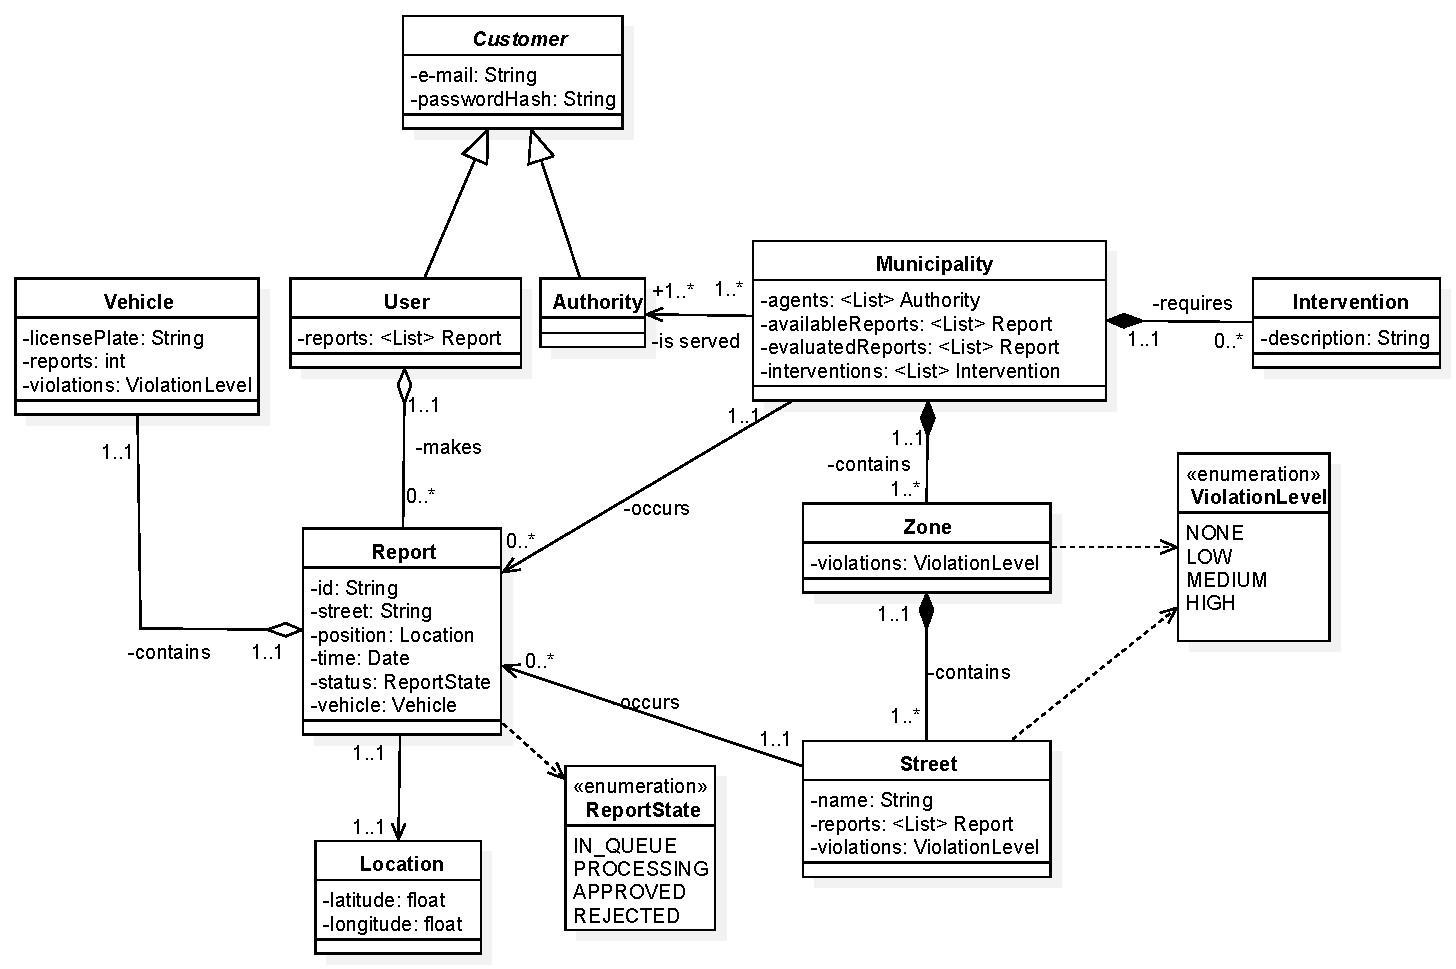
\includegraphics [scale = 0.7, center]{uml}
				\caption{UML diagram of the model}
		\end{figure}

		\section{Selected architectural styles and patterns}
<<<<<<< HEAD
		\newpage
=======
			\subsection{RESTful architecture}
	REST is an architectural style that matches the needs for developing this application: in particular, it positively affects
some properties of the system, such as performance, scalability, modifiability of components, portability and reliability. To obtain this proporties, the REST's architectural main constraints must be followed:
\begin{itemize}
	\item{Client-server}: this principle is natural for the objectives of the application: the user interface must be separated (logically and phisically) from the backend of the application.
	\item{Stateless}: the client-server communication is constrained by no client context being stored on the server between requests. Each request from any client contains all the information necessary to accomplish the request, and the session state is held in the client. The client begins sending requests when it is ready to make the transition to a new state.
	\item{Cacheable}: clients  responses from the server, that has to define them as cacheable or not to prevent clients storing the wrong information. Well-managed caching partially or completely eliminates some client-server interactions, further improving scalability and performance.
	\item{Layered}: the client doesn't know if it's talking with an intermediate or the actual server. So if a proxy or load balancer is placed between the client and server, it won't affect their communications.. Intermediary servers can improve system scalability by enabling load balancing and by providing shared caches. Also, security can be added as a layer on top of the web services, and then clearly separate business logic from security logic.
	\item{Uniform interface}: It simplifies and decouples the architecture, which enables each part to evolve independently. The four constraints for this uniform interface are:
	\begin{itemize}
		\item{Resource identification in requests}: the resources themselves are conceptually separate from the representations that are returned to the client. For example, the server could send data from its database as HTML or XML, none of which are the server's internal representation.
		\item{Resource manipulation through representations}: when a client holds a representation of a resource, including any metadata attached, it has enough information to modify or delete the resource.
		\item{Self-descriptive messages}: each message includes enough information to describe how to process the message.
		\item{Hypermedia as the engine of application state}: a REST client should be able to use server-provided links dynamically to discover all the available actions and resources it needs. As access proceeds, the server responds with text that includes hyperlinks to other actions that are currently available. There is no need for the client to be hard-coded with information regarding the structure or dynamics of the application.
	\end{itemize}
	\end{itemize}
\subsection{Three-tier architecture}
The user interface (presentation tier), functional process logic (application tier) and data access tiers are developed and maintained as independent modules on separate platforms. Apart from the usual advantages of modular software with well-defined interfaces, the three-tier architecture is intended to allow any of the three tiers to be upgraded or replaced independently in response to changes in requirements or technology. For example, a change of operating system in the presentation tier would only affect the user interface code. The other main benefits of the three-tier architecture have been alreday explained in chapter 2.
\subsection{Model-view-controller pattern}
To split the internal representation of information from how it is presented to the user, this pattern divides the application into multiple layers of functionalities: 
\begin{itemize}
\item{Model}: it is the application's dynamic data structure, independent of the user interface. It directly manages the data, logic and rules of the application;
\item{View}: represents the visualization of the data the model contains;
\item{Controller}: controls the data flow into model objects and updates the view whenever data changes. It keeps view and model separate.
\end{itemize}
The main benefits of this pattern are cohesion, low coupling, ease of modification and simultaneous development of the application.

>>>>>>> 062e3b0e4afaf0edc8a9973b1149c0f60bfa88f3
		\section{Other design decisions}
			\subsection{Client}
				A thin client is characterized by the fact that it is primarily designed to communicate with a server: its features 
				are produced by servers. We opted for a thin client to maintain the line of thought underlined till now; this
				design decision also made easier the usage of a MVC design pattern.\\
				Indeed, this allows us to have an architecture in which the real business logic is implemented on the server.
				The centralization of data management methods allows to have a completely thin client, because in case the
				device is off line, the app cannot be used. This choice involves a lighter executive application on the users'
				mobile devices giving them a better experience, furthermore thin clients are strictly dependent on a network 
				connection, and in our case this is not an issue, since the application was conceived to operate most 
				of the time online.\\
			\subsection{DBMS}
				Relational databases are a good choice when there is the need to deal with several transactions and 
				when the data are linked by some relationships (users, reports, authorities etc.). Since there is no need for
				data analysis with different granularity, it was decided not to use non-relational databases, so as to maintain
				high performance with a reasonable saving of memory.
	%end of second chapter

	\chapter{User interfaces design}
	In chapter 3 of the RASD document some screenshots from the user interface were shown. This chapter describes the navigation in the user interface, both for the users and the authorities. The following UX diagrams refer to the mockups shown in the RASD, which are only the most relevant of the following.
	\section{User}
		\begin{figure}[H]
				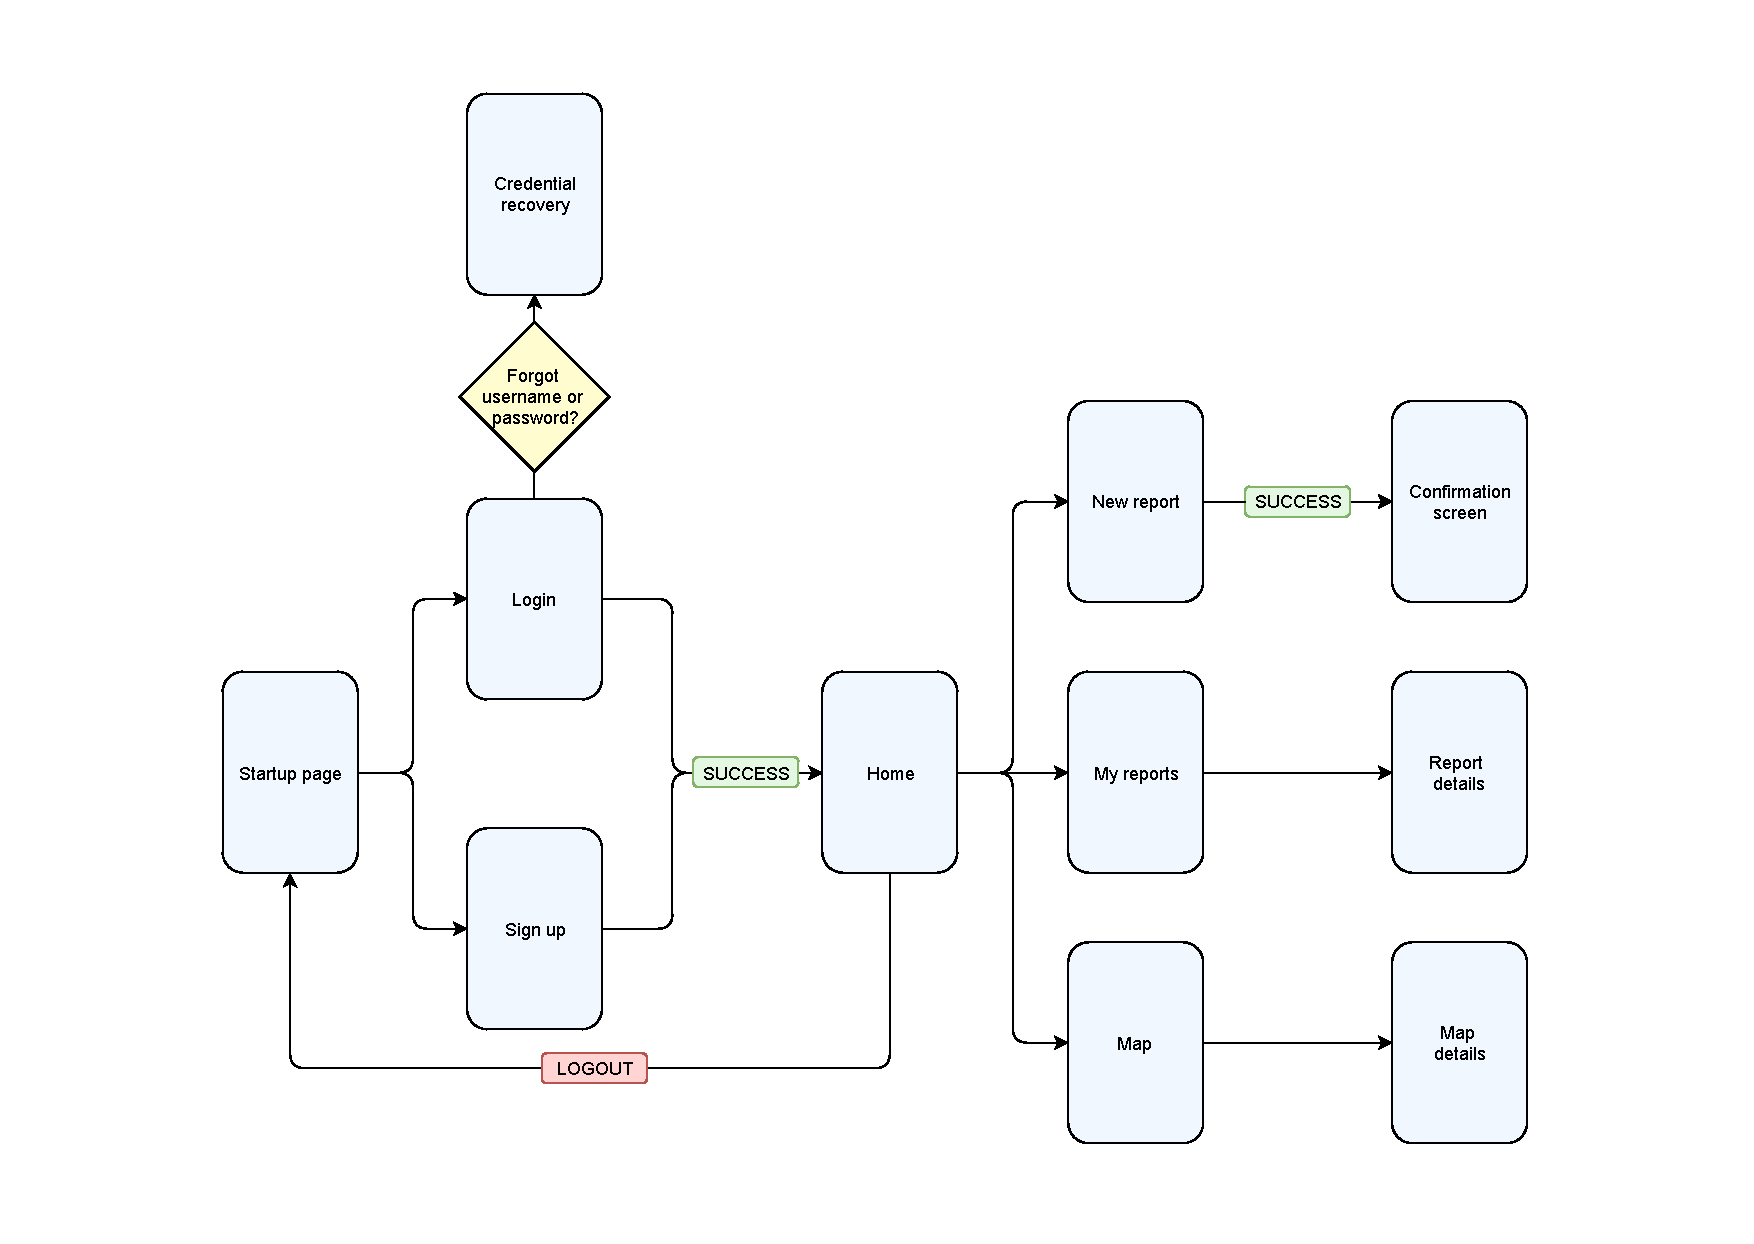
\includegraphics[scale = 0.65, center]{userux}
				\caption{UX diagram - user}
		\end{figure}
	\section{Authority}
		\begin{figure}[H]
				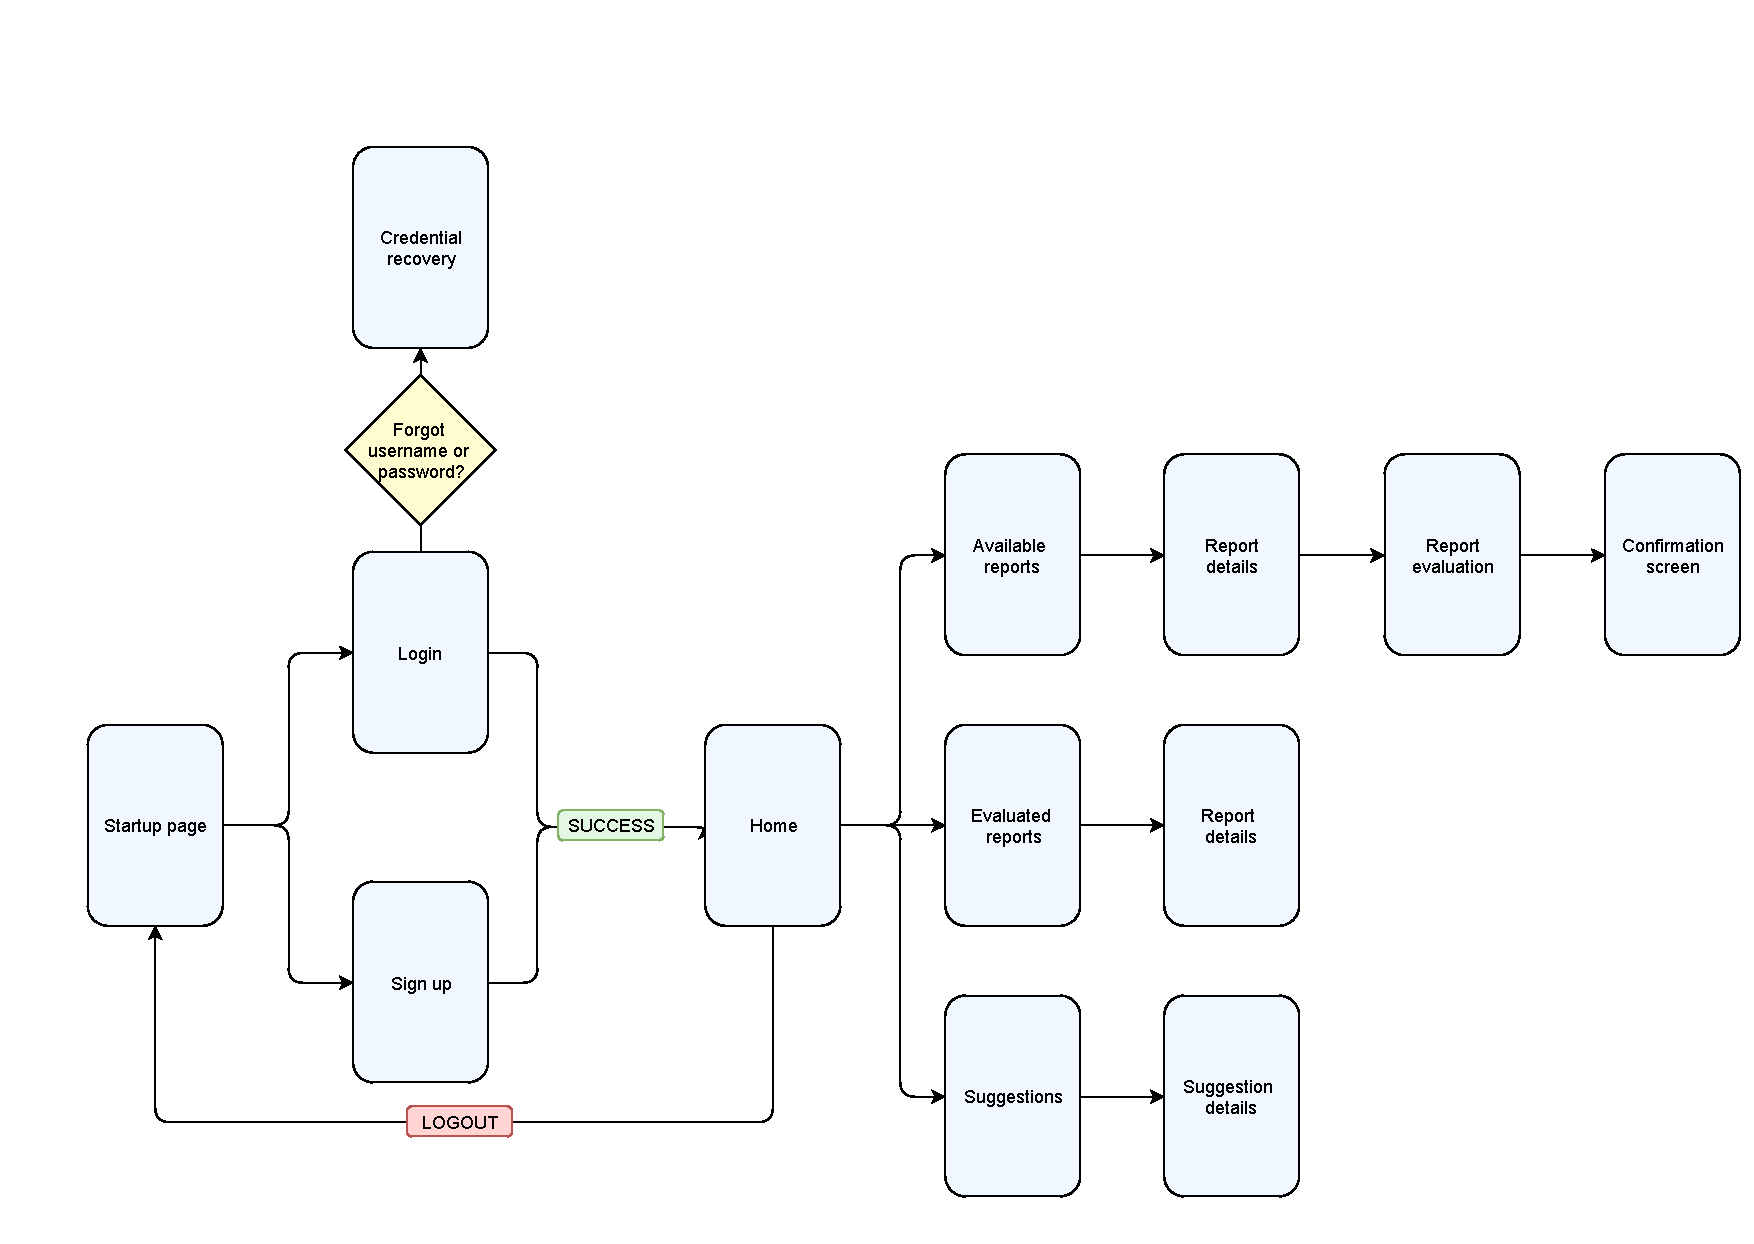
\includegraphics[scale = 0.6, center]{authorityux}
				\caption{UX diagram - authority}
		\end{figure}
	%end of third chapter

	\chapter{Requirements Traceability}
	Chapter 3 of the RASD presented the functional requirements necessary
	to guarantee the goals of the application: this chapter shows how every
	component of the system contributes to satisfy them. For each of the requirements,
	all the involved components in the application server are listed and their function
	is explained.
	\begin{itemize}
	\item\textbf{R1}: Registration must be allowed only entering a valid e-mail address that is not already associated to an existing SafeStreets account.
		\begin{itemize}
		\item\textbf{SignUpManager}: Checks if the e-mail address is already in the DB. In case of sign up, if the address already exists, the request is refused.
		In case of login, checks if the password hashes correspond.
		\end{itemize}
		
	\item\textbf{R2}: Registration must be allowed only entering a password that satisfies the safety conditions.

		This check is made by the client, since the application server can never receive a password as plaintext. Moreover, it is impossible to determine whether
		a string satisfies the safety conditions by reading its hash.
		
	\item\textbf{R3}: The system must store the hash of every password, using a safe cryptographic hash function.

		As said above, the encription must be made by the mobile application, which computes the hash of the password using a safe cryptografic hash function, like one of the SHA-3 family. For what concerns the application server components:
		\begin{itemize}
		\item\textbf{SignUpManager}: Forwards the received hash (computed by the mobile app) to the DB.
		\end{itemize}
		
	\item\textbf{R4}: The system must check if the location of the report belongs to some municipality exploiting SafeStreets.
		\begin{itemize}
		\item\textbf{ReportManager}: Retrieves the position from the report
		\item\textbf{PositionManager}: Retrieves the street given the position, exploiting Google Maps APIs		
		\item\textbf{ReportManager}: Checks in the DB if the street belongs to some registered municipality.
		\end{itemize}
	
	\item\textbf{R5}: The system must add the right date, time and street of the violation to the data provided by the user.

		All this information is added by the mobile app, which exploits Google Maps APIs as well. Date and time are provided by the OS of the device.
		
	\item\textbf{R6}: The system must correctly read the license plate given a picture attached to a report.
		\begin{itemize}
		\item\textbf{ReportManager}: Retrieves the picture attached to the report
		\item\textbf{OCRManager}: Given the picture of the violation, recognizes the license plate by running an OCS algorithm. This is made by the server to
		respect the thin client architecture.
		\end{itemize}	
		
	\item\textbf{R7}: The system must exploit Google Maps APIs to show to the user the map of the violations.

		This is another requirement fulfilled by the mobile application, which will display the map thanks to Google Maps APIs. The streets are shown with different
		colours, as will be explained in R8.
			
	\item\textbf{R8}: The system must show the right colors on the map, given the number of approved reports for each street.
		\begin{itemize}
		\item\textbf{MapsManager}: Given a set of streets, performs queries in the DB, in order to retrieve the number of violation for each of the streets. Then returns
		the color to highlight the street with, according to rules that associate no color to the streets with less violations and red to the ones with the most violations.
		\end{itemize}
			
	\item\textbf{R9}: When a license plate is recognized, the system must show the number of approved reports for that car.
		\begin{itemize}
		\item\textbf{ReportManager}: Once the string is obtained from the OCRManager, checks if in the DB are present some violations committed by the same vehicle. 
		\end{itemize}
			
	\item\textbf{R10}: If the same violation is reported twice, it counts only one time on the map.
		\begin{itemize}
		\item\textbf{ReportManager}: Checks if in the DB is already present an identical violation, reported in the last 24 hours.
		\end{itemize}
			
	\item\textbf{R11}: The system must assign to each report a unique identification number.
		\begin{itemize}
		\item\textbf{ReportManager}: Assigns the unique identification number to each report.
		\end{itemize}
			
	\item\textbf{R12}: Registration must be allowed only entering a valid identification number that is not already associated to an existing SafeStreets account.
		\begin{itemize}
		\item\textbf{SignUpManager}: Checks if in the DB the same identification number is already present.
		\end{itemize}
			
	\item\textbf{R13}: The system must guarantee that each municipality is covered by at least one authority.

		This check is done at data access level, implementing in DB a rule that requires at least one assigned authority for each municipality.
			
	\item\textbf{R14}: The system must notify the authorities when a new report is available.
		\begin{itemize}
		\item\textbf{ReportManager}: After succesfully inserting a new report in the DB, calls the NotificationManager.
		\item\textbf{NotificationManager}: Alerts all the agents assigned to the municipality of the new report.
		\end{itemize}
			
	\item\textbf{R15}: The system must suggest a possible intervention to the authorities of a municipality, according on the number of each type of violation.
		\begin{itemize}
		\item\textbf{RecommendationManager}: Checks every day if the Recommender system has some suggestions.		
		\item\textbf{NotificationManager}: Alerts all the agents assigned to the municipality for which a new intervention is suggested.
		\end{itemize}
			
	\item\textbf{R16}: Login must be allowed only if both e-mail address and password are correct.
		\begin{itemize}
		\item\textbf{LogInManager}: Checks if the e-mail address is already in the DB, then if the password hash matches.
		\end{itemize}
	\end{itemize}
	%end of fourth chapter

	\chapter{Implementation, Integration and Test plan}
		\section{Implementation and test plan}
			To facilitate development, the system has been divided into subsystems, each of which corresponds to one of the
			above mentioned managers. They will be developed individually with a bottom-up approach and the order will be
			imposed by their importance to the systems (how many sub-systems are depending from it) and for the customers.
			After the development of each subsystem they will be tested to check the correctness and then will be executed
			some integration tests. The system will use also some external systems, in particular Google maps to have maps
			always updated and a dbms to store all the data.
			\begin{table}[H]
				\rowcolors{2}{gray!25}{white}	
				\centering
				\begin{tabular}[width = \textwidth, position = center]{|c|c|c|}
					\hline
					Subsystem & Importance for customers & Importance for development\\
					\hline
					\hline
					Sign-up \& Login manager & Low & High\\
					\hline
					Report manager & High & High\\
					\hline
					Maps Manager & High & Low\\
					\hline
					History & High & Low\\
					\hline
					Evaluate & High & High\\
					\hline
					Suggestion & Medium & Medium\\
					\hline
					Notification manager & Low & Low\\
					\hline
					Position Manager & Low & High\\
					\hline
				\end{tabular}
				\label{tab: }
			\end{table}
			\newpage
			It is important to stress that the reports and evaluation functionalities has to be developed and tested
			as a first step because all the others functionalities relies on these two (except the functionalities for the suggestion
			about improve the security on the streets).
			\begin{itemize}
				\item \textbf{Sign up \& login manager:} even if these two are not a core functionality of the system have a
					great importance in SafeStreets, because some functionality require to keep trace in a unique way of
					who did what (for example history or suggestion); so this part have to be prioritized over the others
					(except ``Evaluate manager" and ``Report manager"). 
				\item \textbf{Report manager:} is one of the core functionalities, has to developed with maximum prioritize
					and tested as soon as possible, probably the more critic aspects are the OCR and the position, in order
					to be developed it needs a functioning ``Position manager", otherwise it will not be possible to convert
					the GPS position into a street name to understand where the traffic violation has been committed.
					Even if the ``Notification manager"  is in theory a sub component of this, its development is not so
					crucial for the correct functioning of the system, so it can be developed in a second moment.  
				\item \textbf{Maps manager:}  this component must be developed after the components necessary to
					ensure the creation and evaluation of reports (``Evaluate manager'' and ``Report manager'). It is not
					particularly important to choose the development order between the ``Map manager'' and ``History
					manager', the important thing is that they are properly developed and integrated before developing
					the other. This allow the use of the ``Visualize map" functionality, and see on the map the streets with
					more car accidents.
				\item \textbf{History manager:}  this component must be developed after the components necessary to
					ensure the creation and evaluation of reports (``Evaluate manager'' and ``Report manager'). It is not
					particularly important to choose the development order between the ``Map manager'' and ``History
					manager', the important thing is that they are properly developed and integrated before developing
					the other. This functionality allow the user to see the chronology of his reports.
				\item \textbf{Evaluate manager:} is the second core functionality of the system. This functionality have to be
					able to correct handle concurrency and various authorities that want to evaluate reports various
					reports at the same time. After the correct development of both the core functionalities a integration
					test is necessary to check the correct functioning of the complete system.  
				\item \textbf{Suggestion manager:} this is completely uncorrelated with the rest of the system, so it would be
					better to develop it as last thing, in this way the focus is on the core functionality of the system and
					the correct integration with the rest of the functionalities.
				\item \textbf{Position manager:} this component allows you to get the road or location on the map of the
					user, it has the maximum priority, indeed it allows the system to understand where the report has been
					made.
				\item \textbf{Notification manager:} this component send notification to the users, it can be developed at
					last, on the top of the complete system because is not a crucial aspect of the core functionalities.
			\end{itemize}
		\section{Integration}
			In the following diagrams we are going to show which components will go through the process of 
			integration for a further clarification. The arrows start from the component which ‘uses’ the other one.
			\subsection{Internal component}
				All the components are implemented and unit tested. Subsequently some components are 
				integrated and the integration is tested as well. 
				\newpage
				\begin{figure}[H]
						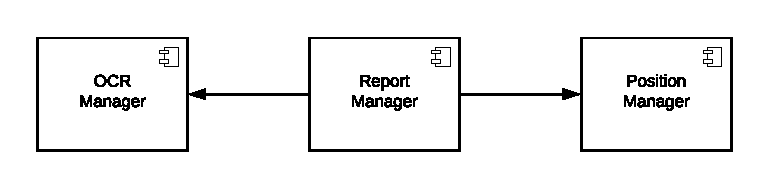
\includegraphics [center]{reportIntegration}
						%\caption{How reports are evaluated}
						\label{fig: interfaces}
				\end{figure}
				\begin{figure}[H]
						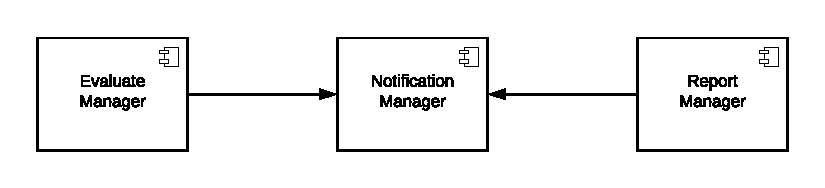
\includegraphics [center]{notificationIntegration}
						%\caption{How reports are evaluated}
						\label{fig: interfaces}
				\end{figure}
				
			
	%end of fifth chapter

	\chapter{Effort Spent}
		\begin{table}[H]
			\rowcolors{2}{gray!25}{white}
			\centering
			\begin{tabular}[width = \textwidth]{|c|c|c|}
				%\rowcolor{gray!50}
				\hline
				Chapter & Frangi (hours) & Fucci (hours)\\
				\hline
				\hline
				Chapter 1 & 1 & 0.5\\
				
				Chapter 2 & 4.5 & 7\\
				
				Chapter 3 & 0.5 & 1.5\\
				
				Chapter 4 & 2 & 4\\
				
				Chapter 5 & 5.5 & 1.5\\
				
				Total hours: & 13.5 & 14.5\\
				\hline
			\end{tabular}
			\label{tab: }
		\end{table}
	%end of sixth chapter
	\chapter{References}
	%end of seventh chapter
\end{document}
